\documentclass[twoside]{book}

% Packages required by doxygen
\usepackage{fixltx2e}
\usepackage{calc}
\usepackage{doxygen}
\usepackage[export]{adjustbox} % also loads graphicx
\usepackage{graphicx}
\usepackage[utf8]{inputenc}
\usepackage{makeidx}
\usepackage{multicol}
\usepackage{multirow}
\PassOptionsToPackage{warn}{textcomp}
\usepackage{textcomp}
\usepackage[nointegrals]{wasysym}
\usepackage[table]{xcolor}

% Font selection
\usepackage[T1]{fontenc}
\usepackage[scaled=.90]{helvet}
\usepackage{courier}
\usepackage{amssymb}
\usepackage{sectsty}
\renewcommand{\familydefault}{\sfdefault}
\allsectionsfont{%
  \fontseries{bc}\selectfont%
  \color{darkgray}%
}
\renewcommand{\DoxyLabelFont}{%
  \fontseries{bc}\selectfont%
  \color{darkgray}%
}
\newcommand{\+}{\discretionary{\mbox{\scriptsize$\hookleftarrow$}}{}{}}

% Page & text layout
\usepackage{geometry}
\geometry{%
  a4paper,%
  top=2.5cm,%
  bottom=2.5cm,%
  left=2.5cm,%
  right=2.5cm%
}
\tolerance=750
\hfuzz=15pt
\hbadness=750
\setlength{\emergencystretch}{15pt}
\setlength{\parindent}{0cm}
\setlength{\parskip}{3ex plus 2ex minus 2ex}
\makeatletter
\renewcommand{\paragraph}{%
  \@startsection{paragraph}{4}{0ex}{-1.0ex}{1.0ex}{%
    \normalfont\normalsize\bfseries\SS@parafont%
  }%
}
\renewcommand{\subparagraph}{%
  \@startsection{subparagraph}{5}{0ex}{-1.0ex}{1.0ex}{%
    \normalfont\normalsize\bfseries\SS@subparafont%
  }%
}
\makeatother

% Headers & footers
\usepackage{fancyhdr}
\pagestyle{fancyplain}
\fancyhead[LE]{\fancyplain{}{\bfseries\thepage}}
\fancyhead[CE]{\fancyplain{}{}}
\fancyhead[RE]{\fancyplain{}{\bfseries\leftmark}}
\fancyhead[LO]{\fancyplain{}{\bfseries\rightmark}}
\fancyhead[CO]{\fancyplain{}{}}
\fancyhead[RO]{\fancyplain{}{\bfseries\thepage}}
\fancyfoot[LE]{\fancyplain{}{}}
\fancyfoot[CE]{\fancyplain{}{}}
\fancyfoot[RE]{\fancyplain{}{\bfseries\scriptsize Generated by Doxygen }}
\fancyfoot[LO]{\fancyplain{}{\bfseries\scriptsize Generated by Doxygen }}
\fancyfoot[CO]{\fancyplain{}{}}
\fancyfoot[RO]{\fancyplain{}{}}
\renewcommand{\footrulewidth}{0.4pt}
\renewcommand{\chaptermark}[1]{%
  \markboth{#1}{}%
}
\renewcommand{\sectionmark}[1]{%
  \markright{\thesection\ #1}%
}

% Indices & bibliography
\usepackage{natbib}
\usepackage[titles]{tocloft}
\setcounter{tocdepth}{3}
\setcounter{secnumdepth}{5}
\makeindex

% Hyperlinks (required, but should be loaded last)
\usepackage{ifpdf}
\ifpdf
  \usepackage[pdftex,pagebackref=true]{hyperref}
\else
  \usepackage[ps2pdf,pagebackref=true]{hyperref}
\fi
\hypersetup{%
  colorlinks=true,%
  linkcolor=blue,%
  citecolor=blue,%
  unicode%
}

% Custom commands
\newcommand{\clearemptydoublepage}{%
  \newpage{\pagestyle{empty}\cleardoublepage}%
}

\usepackage{caption}
\captionsetup{labelsep=space,justification=centering,font={bf},singlelinecheck=off,skip=4pt,position=top}

%===== C O N T E N T S =====

\begin{document}

% Titlepage & ToC
\hypersetup{pageanchor=false,
             bookmarksnumbered=true,
             pdfencoding=unicode
            }
\pagenumbering{alph}
\begin{titlepage}
\vspace*{7cm}
\begin{center}%
{\Large My Project }\\
\vspace*{1cm}
{\large Generated by Doxygen 1.8.15}\\
\end{center}
\end{titlepage}
\clearemptydoublepage
\pagenumbering{roman}
\tableofcontents
\clearemptydoublepage
\pagenumbering{arabic}
\hypersetup{pageanchor=true}

%--- Begin generated contents ---
\chapter{Hierarchical Index}
\section{Class Hierarchy}
This inheritance list is sorted roughly, but not completely, alphabetically\+:\begin{DoxyCompactList}
\item \contentsline{section}{binary\+\_\+search}{\pageref{enumbinary__search}}{}
\item \contentsline{section}{binary\+\_\+search\+\_\+tb}{\pageref{enumbinary__search__tb}}{}
\item \contentsline{section}{dp\+\_\+ram}{\pageref{enumdp__ram}}{}
\item \contentsline{section}{dp\+\_\+ram1}{\pageref{enumdp__ram1}}{}
\item \contentsline{section}{packet\+\_\+parser}{\pageref{enumpacket__parser}}{}
\item \contentsline{section}{packet\+\_\+parser\+\_\+top}{\pageref{enumpacket__parser__top}}{}
\begin{DoxyCompactList}
\item \contentsline{section}{packet\+\_\+parser\+\_\+top\+\_\+tb}{\pageref{enumpacket__parser__top__tb}}{}
\end{DoxyCompactList}
\end{DoxyCompactList}

\chapter{Class Index}
\section{Class List}
Here are the classes, structs, unions and interfaces with brief descriptions\+:\begin{DoxyCompactList}
\item\contentsline{section}{\mbox{\hyperlink{enumbinary__search}{binary\+\_\+search}} }{\pageref{enumbinary__search}}{}
\item\contentsline{section}{\mbox{\hyperlink{enumbinary__search__tb}{binary\+\_\+search\+\_\+tb}} }{\pageref{enumbinary__search__tb}}{}
\item\contentsline{section}{\mbox{\hyperlink{enumdp__ram}{dp\+\_\+ram}} }{\pageref{enumdp__ram}}{}
\item\contentsline{section}{\mbox{\hyperlink{enumdp__ram1}{dp\+\_\+ram1}} }{\pageref{enumdp__ram1}}{}
\item\contentsline{section}{\mbox{\hyperlink{enumpacket__parser}{packet\+\_\+parser}} }{\pageref{enumpacket__parser}}{}
\item\contentsline{section}{\mbox{\hyperlink{enumpacket__parser__top}{packet\+\_\+parser\+\_\+top}} }{\pageref{enumpacket__parser__top}}{}
\item\contentsline{section}{\mbox{\hyperlink{enumpacket__parser__top__tb}{packet\+\_\+parser\+\_\+top\+\_\+tb}} }{\pageref{enumpacket__parser__top__tb}}{}
\end{DoxyCompactList}

\chapter{File Index}
\section{File List}
Here is a list of all files with brief descriptions\+:\begin{DoxyCompactList}
\item\contentsline{section}{\mbox{\hyperlink{binary__search_8v}{binary\+\_\+search.\+v}} }{\pageref{binary__search_8v}}{}
\item\contentsline{section}{\mbox{\hyperlink{binary__search__tb_8v}{binary\+\_\+search\+\_\+tb.\+v}} }{\pageref{binary__search__tb_8v}}{}
\item\contentsline{section}{\mbox{\hyperlink{dp__ram_8v}{dp\+\_\+ram.\+v}} }{\pageref{dp__ram_8v}}{}
\item\contentsline{section}{\mbox{\hyperlink{dp__ram1_8v}{dp\+\_\+ram1.\+v}} }{\pageref{dp__ram1_8v}}{}
\item\contentsline{section}{\mbox{\hyperlink{packet__parser_8v}{packet\+\_\+parser.\+v}} }{\pageref{packet__parser_8v}}{}
\item\contentsline{section}{\mbox{\hyperlink{packet__parser__top_8v}{packet\+\_\+parser\+\_\+top.\+v}} }{\pageref{packet__parser__top_8v}}{}
\item\contentsline{section}{\mbox{\hyperlink{packet__parser__top__tb_8v}{packet\+\_\+parser\+\_\+top\+\_\+tb.\+v}} }{\pageref{packet__parser__top__tb_8v}}{}
\end{DoxyCompactList}

\chapter{Class Documentation}
\hypertarget{enumbinary__search}{}\section{binary\+\_\+search Enum Reference}
\label{enumbinary__search}\index{binary\+\_\+search@{binary\+\_\+search}}


The documentation for this enum was generated from the following file\+:\begin{DoxyCompactItemize}
\item 
\mbox{\hyperlink{binary__search_8v}{binary\+\_\+search.\+v}}\end{DoxyCompactItemize}

\hypertarget{enumbinary__search__tb}{}\section{binary\+\_\+search\+\_\+tb Enum Reference}
\label{enumbinary__search__tb}\index{binary\+\_\+search\+\_\+tb@{binary\+\_\+search\+\_\+tb}}
\subsection*{Static Public Member Functions}
\begin{DoxyCompactItemize}
\item 
\mbox{\hyperlink{enumbinary__search__tb_a75170e052c291ff4de20a9154177d7ab}{P\+R\+O\+C\+E\+S\+S\+\_\+0}} Clk
\item 
\mbox{\hyperlink{enumbinary__search__tb_a663d8c3c055c8dbfef5b94aeffb17fec}{P\+R\+O\+C\+E\+S\+S\+\_\+1}} Clk
\end{DoxyCompactItemize}
\subsection*{Public Attributes}
\begin{DoxyCompactItemize}
\item 
\mbox{\hyperlink{enumbinary__search__tb_a148adc223b3ec1ebf1a9d3014bba5c57}{Clk}} reg
\item 
\mbox{\hyperlink{enumbinary__search__tb_ad64af76bd3572600605115944fe0ddeb}{Rst}} reg
\item 
\mbox{\hyperlink{enumbinary__search__tb_a966aad5e0c678340650456fee3ae4392}{D\+E\+P\+TH}} \textquotesingle{}d1024
\item 
\mbox{\hyperlink{enumbinary__search__tb_a4320519c9374f2c2755d18e3f83abe38}{D\+A\+T\+A\+\_\+\+W\+I\+D\+TH}} \textquotesingle{}d32
\item 
\mbox{\hyperlink{enumbinary__search__tb_a756353f91e17615905867350b7df2178}{I\+D\+LE}} 3 \textquotesingle{}d0
\item 
\mbox{\hyperlink{enumbinary__search__tb_ab04344ebfa7778e003bff3b5b90b98b5}{W\+A\+IT}} 3 \textquotesingle{}d1
\item 
\mbox{\hyperlink{enumbinary__search__tb_a48be18b536c71939fee1bc175ddfe82f}{R\+E\+Q\+U\+ST}} 3 \textquotesingle{}d2
\item 
\mbox{\hyperlink{enumbinary__search__tb_a3bdf46b2b8703a5293bb1322d4802039}{C\+O\+M\+P\+A\+RE}} 3 \textquotesingle{}d3
\item 
\mbox{[}0\+:D\+E\+P\+TH-\/1\mbox{]} \mbox{\hyperlink{enumbinary__search__tb_a1f84d0ccad171ddd61f482601523e35b}{mem}} reg\mbox{[}D\+A\+T\+A\+\_\+\+W\+I\+D\+TH-\/1\+:0\mbox{]}
\item 
\mbox{\hyperlink{enumbinary__search__tb_a55f9f2f8be34929a07a9cbd51b0077ef}{request\+\_\+key}} reg\mbox{[}D\+A\+T\+A\+\_\+\+W\+I\+D\+TH-\/1\+:0\mbox{]}
\item 
\mbox{\hyperlink{enumbinary__search__tb_a915112263d36b38ff53acdf2a4f1c7e7}{sw\+\_\+state}} reg\mbox{[}1\+:0\mbox{]}
\item 
\mbox{\hyperlink{enumbinary__search__tb_a5dea527f6196d0f38b066d000f02ed02}{req\+\_\+state}} reg\mbox{[}1\+:0\mbox{]}
\item 
\mbox{\hyperlink{enumbinary__search__tb_a108c2786d7b262af34cfd3b13d923d82}{j}} reg\mbox{[} \$clog2\+D\+E\+P\+TH-\/1\+:0\mbox{]}
\item 
\mbox{\hyperlink{enumbinary__search__tb_a7d2f566ab297925c822fd0dceb40a4a6}{test\+\_\+index}} reg\mbox{[} \$clog2\+D\+E\+P\+TH-\/1\+:0\mbox{]}
\item 
\mbox{\hyperlink{enumbinary__search__tb_a2078db9c91f7c7f69755bfb791850765}{test\+\_\+index\+\_\+latched}} reg\mbox{[} \$clog2\+D\+E\+P\+TH-\/1\+:0\mbox{]}
\item 
\mbox{\hyperlink{enumbinary__search__tb_add4396c2f76da13db52c737030c183af}{response\+\_\+index}} wire\mbox{[} \$clog2\+D\+E\+P\+TH-\/1\+:0\mbox{]}
\item 
\mbox{\hyperlink{enumbinary__search__tb_aedbfae3fc907ebe52e22fe368bb8998f}{request\+\_\+key\+\_\+valid}} reg
\item 
\mbox{\hyperlink{enumbinary__search__tb_ab7c6c4f4e41027e2ab46a9531402fe66}{wait\+\_\+count}} reg\mbox{[}2\+:0\mbox{]}
\item 
\mbox{\hyperlink{enumbinary__search__tb_a19628ba8402e042b55f2c844586edfb9}{cpu\+\_\+data}} reg\mbox{[}D\+A\+T\+A\+\_\+\+W\+I\+D\+TH-\/1\+:0\mbox{]}
\item 
\mbox{\hyperlink{enumbinary__search__tb_a5e0629d67883cbd861305185e6af3cbe}{cpu\+\_\+addr}} reg\mbox{[} \$clog2\+D\+E\+P\+TH-\/1\+:0\mbox{]}
\item 
\mbox{\hyperlink{enumbinary__search__tb_aab06c31ae3c20c2728995ed2bdc4d938}{cpu\+\_\+wr}} reg
\item 
\mbox{\hyperlink{enumbinary__search__tb_a757f69c7d26265dc1e79f5297b6134ed}{cpu\+\_\+rd}} reg
\item 
\mbox{\hyperlink{enumbinary__search__tb_a5117977ac113d88efb1ecefae610b4b6}{init\+\_\+done}} reg
\end{DoxyCompactItemize}


\subsection{Member Function Documentation}
\mbox{\Hypertarget{enumbinary__search__tb_a75170e052c291ff4de20a9154177d7ab}\label{enumbinary__search__tb_a75170e052c291ff4de20a9154177d7ab}} 
\index{binary\+\_\+search\+\_\+tb@{binary\+\_\+search\+\_\+tb}!P\+R\+O\+C\+E\+S\+S\+\_\+0@{P\+R\+O\+C\+E\+S\+S\+\_\+0}}
\index{P\+R\+O\+C\+E\+S\+S\+\_\+0@{P\+R\+O\+C\+E\+S\+S\+\_\+0}!binary\+\_\+search\+\_\+tb@{binary\+\_\+search\+\_\+tb}}
\subsubsection{\texorpdfstring{P\+R\+O\+C\+E\+S\+S\+\_\+0()}{PROCESS\_0()}}
{\footnotesize\ttfamily \hspace{0.3cm}}

\mbox{\Hypertarget{enumbinary__search__tb_a663d8c3c055c8dbfef5b94aeffb17fec}\label{enumbinary__search__tb_a663d8c3c055c8dbfef5b94aeffb17fec}} 
\index{binary\+\_\+search\+\_\+tb@{binary\+\_\+search\+\_\+tb}!P\+R\+O\+C\+E\+S\+S\+\_\+1@{P\+R\+O\+C\+E\+S\+S\+\_\+1}}
\index{P\+R\+O\+C\+E\+S\+S\+\_\+1@{P\+R\+O\+C\+E\+S\+S\+\_\+1}!binary\+\_\+search\+\_\+tb@{binary\+\_\+search\+\_\+tb}}
\subsubsection{\texorpdfstring{P\+R\+O\+C\+E\+S\+S\+\_\+1()}{PROCESS\_1()}}
{\footnotesize\ttfamily \hspace{0.3cm}}



\subsection{Member Data Documentation}
\mbox{\Hypertarget{enumbinary__search__tb_a148adc223b3ec1ebf1a9d3014bba5c57}\label{enumbinary__search__tb_a148adc223b3ec1ebf1a9d3014bba5c57}} 
\index{binary\+\_\+search\+\_\+tb@{binary\+\_\+search\+\_\+tb}!Clk@{Clk}}
\index{Clk@{Clk}!binary\+\_\+search\+\_\+tb@{binary\+\_\+search\+\_\+tb}}
\subsubsection{\texorpdfstring{Clk}{Clk}}
{\footnotesize\ttfamily \mbox{\hyperlink{enumbinary__search__tb_a148adc223b3ec1ebf1a9d3014bba5c57}{Clk}} {\bfseries \textcolor{vhdlchar}{ }} \hspace{0.3cm}}

\mbox{\Hypertarget{enumbinary__search__tb_a915112263d36b38ff53acdf2a4f1c7e7}\label{enumbinary__search__tb_a915112263d36b38ff53acdf2a4f1c7e7}} 
\index{binary\+\_\+search\+\_\+tb@{binary\+\_\+search\+\_\+tb}!sw\+\_\+state@{sw\+\_\+state}}
\index{sw\+\_\+state@{sw\+\_\+state}!binary\+\_\+search\+\_\+tb@{binary\+\_\+search\+\_\+tb}}
\subsubsection{\texorpdfstring{sw\+\_\+state}{sw\_state}}
{\footnotesize\ttfamily \mbox{\hyperlink{enumbinary__search__tb_a915112263d36b38ff53acdf2a4f1c7e7}{sw\+\_\+state}} {\bfseries \textcolor{vhdlchar}{ }} \hspace{0.3cm}}

\mbox{\Hypertarget{enumbinary__search__tb_a5dea527f6196d0f38b066d000f02ed02}\label{enumbinary__search__tb_a5dea527f6196d0f38b066d000f02ed02}} 
\index{binary\+\_\+search\+\_\+tb@{binary\+\_\+search\+\_\+tb}!req\+\_\+state@{req\+\_\+state}}
\index{req\+\_\+state@{req\+\_\+state}!binary\+\_\+search\+\_\+tb@{binary\+\_\+search\+\_\+tb}}
\subsubsection{\texorpdfstring{req\+\_\+state}{req\_state}}
{\footnotesize\ttfamily \mbox{\hyperlink{enumbinary__search__tb_a5dea527f6196d0f38b066d000f02ed02}{req\+\_\+state}} {\bfseries \textcolor{vhdlchar}{ }} \hspace{0.3cm}}

\mbox{\Hypertarget{enumbinary__search__tb_a108c2786d7b262af34cfd3b13d923d82}\label{enumbinary__search__tb_a108c2786d7b262af34cfd3b13d923d82}} 
\index{binary\+\_\+search\+\_\+tb@{binary\+\_\+search\+\_\+tb}!j@{j}}
\index{j@{j}!binary\+\_\+search\+\_\+tb@{binary\+\_\+search\+\_\+tb}}
\subsubsection{\texorpdfstring{j}{j}}
{\footnotesize\ttfamily \mbox{\hyperlink{enumbinary__search__tb_a108c2786d7b262af34cfd3b13d923d82}{j}} {\bfseries \textcolor{vhdlchar}{ }} \hspace{0.3cm}}

\mbox{\Hypertarget{enumbinary__search__tb_a7d2f566ab297925c822fd0dceb40a4a6}\label{enumbinary__search__tb_a7d2f566ab297925c822fd0dceb40a4a6}} 
\index{binary\+\_\+search\+\_\+tb@{binary\+\_\+search\+\_\+tb}!test\+\_\+index@{test\+\_\+index}}
\index{test\+\_\+index@{test\+\_\+index}!binary\+\_\+search\+\_\+tb@{binary\+\_\+search\+\_\+tb}}
\subsubsection{\texorpdfstring{test\+\_\+index}{test\_index}}
{\footnotesize\ttfamily \mbox{\hyperlink{enumbinary__search__tb_a7d2f566ab297925c822fd0dceb40a4a6}{test\+\_\+index}} {\bfseries \textcolor{vhdlchar}{ }} \hspace{0.3cm}}

\mbox{\Hypertarget{enumbinary__search__tb_a2078db9c91f7c7f69755bfb791850765}\label{enumbinary__search__tb_a2078db9c91f7c7f69755bfb791850765}} 
\index{binary\+\_\+search\+\_\+tb@{binary\+\_\+search\+\_\+tb}!test\+\_\+index\+\_\+latched@{test\+\_\+index\+\_\+latched}}
\index{test\+\_\+index\+\_\+latched@{test\+\_\+index\+\_\+latched}!binary\+\_\+search\+\_\+tb@{binary\+\_\+search\+\_\+tb}}
\subsubsection{\texorpdfstring{test\+\_\+index\+\_\+latched}{test\_index\_latched}}
{\footnotesize\ttfamily \mbox{\hyperlink{enumbinary__search__tb_a2078db9c91f7c7f69755bfb791850765}{test\+\_\+index\+\_\+latched}} {\bfseries \textcolor{vhdlchar}{ }} \hspace{0.3cm}}

\mbox{\Hypertarget{enumbinary__search__tb_add4396c2f76da13db52c737030c183af}\label{enumbinary__search__tb_add4396c2f76da13db52c737030c183af}} 
\index{binary\+\_\+search\+\_\+tb@{binary\+\_\+search\+\_\+tb}!response\+\_\+index@{response\+\_\+index}}
\index{response\+\_\+index@{response\+\_\+index}!binary\+\_\+search\+\_\+tb@{binary\+\_\+search\+\_\+tb}}
\subsubsection{\texorpdfstring{response\+\_\+index}{response\_index}}
{\footnotesize\ttfamily \mbox{\hyperlink{enumbinary__search__tb_add4396c2f76da13db52c737030c183af}{response\+\_\+index}} {\bfseries \textcolor{vhdlchar}{ }} \hspace{0.3cm}}

\mbox{\Hypertarget{enumbinary__search__tb_aedbfae3fc907ebe52e22fe368bb8998f}\label{enumbinary__search__tb_aedbfae3fc907ebe52e22fe368bb8998f}} 
\index{binary\+\_\+search\+\_\+tb@{binary\+\_\+search\+\_\+tb}!request\+\_\+key\+\_\+valid@{request\+\_\+key\+\_\+valid}}
\index{request\+\_\+key\+\_\+valid@{request\+\_\+key\+\_\+valid}!binary\+\_\+search\+\_\+tb@{binary\+\_\+search\+\_\+tb}}
\subsubsection{\texorpdfstring{request\+\_\+key\+\_\+valid}{request\_key\_valid}}
{\footnotesize\ttfamily \mbox{\hyperlink{enumbinary__search__tb_aedbfae3fc907ebe52e22fe368bb8998f}{request\+\_\+key\+\_\+valid}} {\bfseries \textcolor{vhdlchar}{ }} \hspace{0.3cm}}

\mbox{\Hypertarget{enumbinary__search__tb_ab7c6c4f4e41027e2ab46a9531402fe66}\label{enumbinary__search__tb_ab7c6c4f4e41027e2ab46a9531402fe66}} 
\index{binary\+\_\+search\+\_\+tb@{binary\+\_\+search\+\_\+tb}!wait\+\_\+count@{wait\+\_\+count}}
\index{wait\+\_\+count@{wait\+\_\+count}!binary\+\_\+search\+\_\+tb@{binary\+\_\+search\+\_\+tb}}
\subsubsection{\texorpdfstring{wait\+\_\+count}{wait\_count}}
{\footnotesize\ttfamily \mbox{\hyperlink{enumbinary__search__tb_ab7c6c4f4e41027e2ab46a9531402fe66}{wait\+\_\+count}} {\bfseries \textcolor{vhdlchar}{ }} \hspace{0.3cm}}

\mbox{\Hypertarget{enumbinary__search__tb_a19628ba8402e042b55f2c844586edfb9}\label{enumbinary__search__tb_a19628ba8402e042b55f2c844586edfb9}} 
\index{binary\+\_\+search\+\_\+tb@{binary\+\_\+search\+\_\+tb}!cpu\+\_\+data@{cpu\+\_\+data}}
\index{cpu\+\_\+data@{cpu\+\_\+data}!binary\+\_\+search\+\_\+tb@{binary\+\_\+search\+\_\+tb}}
\subsubsection{\texorpdfstring{cpu\+\_\+data}{cpu\_data}}
{\footnotesize\ttfamily \mbox{\hyperlink{enumbinary__search__tb_a19628ba8402e042b55f2c844586edfb9}{cpu\+\_\+data}} {\bfseries \textcolor{vhdlchar}{ }} \hspace{0.3cm}}

\mbox{\Hypertarget{enumbinary__search__tb_a5e0629d67883cbd861305185e6af3cbe}\label{enumbinary__search__tb_a5e0629d67883cbd861305185e6af3cbe}} 
\index{binary\+\_\+search\+\_\+tb@{binary\+\_\+search\+\_\+tb}!cpu\+\_\+addr@{cpu\+\_\+addr}}
\index{cpu\+\_\+addr@{cpu\+\_\+addr}!binary\+\_\+search\+\_\+tb@{binary\+\_\+search\+\_\+tb}}
\subsubsection{\texorpdfstring{cpu\+\_\+addr}{cpu\_addr}}
{\footnotesize\ttfamily \mbox{\hyperlink{enumbinary__search__tb_a5e0629d67883cbd861305185e6af3cbe}{cpu\+\_\+addr}} {\bfseries \textcolor{vhdlchar}{ }} \hspace{0.3cm}}

\mbox{\Hypertarget{enumbinary__search__tb_ad64af76bd3572600605115944fe0ddeb}\label{enumbinary__search__tb_ad64af76bd3572600605115944fe0ddeb}} 
\index{binary\+\_\+search\+\_\+tb@{binary\+\_\+search\+\_\+tb}!Rst@{Rst}}
\index{Rst@{Rst}!binary\+\_\+search\+\_\+tb@{binary\+\_\+search\+\_\+tb}}
\subsubsection{\texorpdfstring{Rst}{Rst}}
{\footnotesize\ttfamily \mbox{\hyperlink{enumbinary__search__tb_ad64af76bd3572600605115944fe0ddeb}{Rst}} {\bfseries \textcolor{vhdlchar}{ }} \hspace{0.3cm}}

\mbox{\Hypertarget{enumbinary__search__tb_aab06c31ae3c20c2728995ed2bdc4d938}\label{enumbinary__search__tb_aab06c31ae3c20c2728995ed2bdc4d938}} 
\index{binary\+\_\+search\+\_\+tb@{binary\+\_\+search\+\_\+tb}!cpu\+\_\+wr@{cpu\+\_\+wr}}
\index{cpu\+\_\+wr@{cpu\+\_\+wr}!binary\+\_\+search\+\_\+tb@{binary\+\_\+search\+\_\+tb}}
\subsubsection{\texorpdfstring{cpu\+\_\+wr}{cpu\_wr}}
{\footnotesize\ttfamily \mbox{\hyperlink{enumbinary__search__tb_aab06c31ae3c20c2728995ed2bdc4d938}{cpu\+\_\+wr}} {\bfseries \textcolor{vhdlchar}{ }} \hspace{0.3cm}}

\mbox{\Hypertarget{enumbinary__search__tb_a757f69c7d26265dc1e79f5297b6134ed}\label{enumbinary__search__tb_a757f69c7d26265dc1e79f5297b6134ed}} 
\index{binary\+\_\+search\+\_\+tb@{binary\+\_\+search\+\_\+tb}!cpu\+\_\+rd@{cpu\+\_\+rd}}
\index{cpu\+\_\+rd@{cpu\+\_\+rd}!binary\+\_\+search\+\_\+tb@{binary\+\_\+search\+\_\+tb}}
\subsubsection{\texorpdfstring{cpu\+\_\+rd}{cpu\_rd}}
{\footnotesize\ttfamily \mbox{\hyperlink{enumbinary__search__tb_a757f69c7d26265dc1e79f5297b6134ed}{cpu\+\_\+rd}} {\bfseries \textcolor{vhdlchar}{ }} \hspace{0.3cm}}

\mbox{\Hypertarget{enumbinary__search__tb_a5117977ac113d88efb1ecefae610b4b6}\label{enumbinary__search__tb_a5117977ac113d88efb1ecefae610b4b6}} 
\index{binary\+\_\+search\+\_\+tb@{binary\+\_\+search\+\_\+tb}!init\+\_\+done@{init\+\_\+done}}
\index{init\+\_\+done@{init\+\_\+done}!binary\+\_\+search\+\_\+tb@{binary\+\_\+search\+\_\+tb}}
\subsubsection{\texorpdfstring{init\+\_\+done}{init\_done}}
{\footnotesize\ttfamily \mbox{\hyperlink{enumbinary__search__tb_a5117977ac113d88efb1ecefae610b4b6}{init\+\_\+done}} {\bfseries \textcolor{vhdlchar}{ }} \hspace{0.3cm}}

\mbox{\Hypertarget{enumbinary__search__tb_a966aad5e0c678340650456fee3ae4392}\label{enumbinary__search__tb_a966aad5e0c678340650456fee3ae4392}} 
\index{binary\+\_\+search\+\_\+tb@{binary\+\_\+search\+\_\+tb}!D\+E\+P\+TH@{D\+E\+P\+TH}}
\index{D\+E\+P\+TH@{D\+E\+P\+TH}!binary\+\_\+search\+\_\+tb@{binary\+\_\+search\+\_\+tb}}
\subsubsection{\texorpdfstring{D\+E\+P\+TH}{DEPTH}}
{\footnotesize\ttfamily \mbox{\hyperlink{enumbinary__search__tb_a966aad5e0c678340650456fee3ae4392}{D\+E\+P\+TH}} {\bfseries \textcolor{vhdlchar}{ }} \hspace{0.3cm}}

\mbox{\Hypertarget{enumbinary__search__tb_a4320519c9374f2c2755d18e3f83abe38}\label{enumbinary__search__tb_a4320519c9374f2c2755d18e3f83abe38}} 
\index{binary\+\_\+search\+\_\+tb@{binary\+\_\+search\+\_\+tb}!D\+A\+T\+A\+\_\+\+W\+I\+D\+TH@{D\+A\+T\+A\+\_\+\+W\+I\+D\+TH}}
\index{D\+A\+T\+A\+\_\+\+W\+I\+D\+TH@{D\+A\+T\+A\+\_\+\+W\+I\+D\+TH}!binary\+\_\+search\+\_\+tb@{binary\+\_\+search\+\_\+tb}}
\subsubsection{\texorpdfstring{D\+A\+T\+A\+\_\+\+W\+I\+D\+TH}{DATA\_WIDTH}}
{\footnotesize\ttfamily \mbox{\hyperlink{enumbinary__search__tb_a4320519c9374f2c2755d18e3f83abe38}{D\+A\+T\+A\+\_\+\+W\+I\+D\+TH}} {\bfseries \textcolor{vhdlchar}{ }} \hspace{0.3cm}}

\mbox{\Hypertarget{enumbinary__search__tb_a756353f91e17615905867350b7df2178}\label{enumbinary__search__tb_a756353f91e17615905867350b7df2178}} 
\index{binary\+\_\+search\+\_\+tb@{binary\+\_\+search\+\_\+tb}!I\+D\+LE@{I\+D\+LE}}
\index{I\+D\+LE@{I\+D\+LE}!binary\+\_\+search\+\_\+tb@{binary\+\_\+search\+\_\+tb}}
\subsubsection{\texorpdfstring{I\+D\+LE}{IDLE}}
{\footnotesize\ttfamily \mbox{\hyperlink{enumbinary__search__tb_a756353f91e17615905867350b7df2178}{I\+D\+LE}} {\bfseries \textcolor{vhdlchar}{ }} \hspace{0.3cm}}

\mbox{\Hypertarget{enumbinary__search__tb_ab04344ebfa7778e003bff3b5b90b98b5}\label{enumbinary__search__tb_ab04344ebfa7778e003bff3b5b90b98b5}} 
\index{binary\+\_\+search\+\_\+tb@{binary\+\_\+search\+\_\+tb}!W\+A\+IT@{W\+A\+IT}}
\index{W\+A\+IT@{W\+A\+IT}!binary\+\_\+search\+\_\+tb@{binary\+\_\+search\+\_\+tb}}
\subsubsection{\texorpdfstring{W\+A\+IT}{WAIT}}
{\footnotesize\ttfamily \mbox{\hyperlink{enumbinary__search__tb_ab04344ebfa7778e003bff3b5b90b98b5}{W\+A\+IT}} {\bfseries \textcolor{vhdlchar}{ }} \hspace{0.3cm}}

\mbox{\Hypertarget{enumbinary__search__tb_a48be18b536c71939fee1bc175ddfe82f}\label{enumbinary__search__tb_a48be18b536c71939fee1bc175ddfe82f}} 
\index{binary\+\_\+search\+\_\+tb@{binary\+\_\+search\+\_\+tb}!R\+E\+Q\+U\+ST@{R\+E\+Q\+U\+ST}}
\index{R\+E\+Q\+U\+ST@{R\+E\+Q\+U\+ST}!binary\+\_\+search\+\_\+tb@{binary\+\_\+search\+\_\+tb}}
\subsubsection{\texorpdfstring{R\+E\+Q\+U\+ST}{REQUST}}
{\footnotesize\ttfamily \mbox{\hyperlink{enumbinary__search__tb_a48be18b536c71939fee1bc175ddfe82f}{R\+E\+Q\+U\+ST}} {\bfseries \textcolor{vhdlchar}{ }} \hspace{0.3cm}}

\mbox{\Hypertarget{enumbinary__search__tb_a3bdf46b2b8703a5293bb1322d4802039}\label{enumbinary__search__tb_a3bdf46b2b8703a5293bb1322d4802039}} 
\index{binary\+\_\+search\+\_\+tb@{binary\+\_\+search\+\_\+tb}!C\+O\+M\+P\+A\+RE@{C\+O\+M\+P\+A\+RE}}
\index{C\+O\+M\+P\+A\+RE@{C\+O\+M\+P\+A\+RE}!binary\+\_\+search\+\_\+tb@{binary\+\_\+search\+\_\+tb}}
\subsubsection{\texorpdfstring{C\+O\+M\+P\+A\+RE}{COMPARE}}
{\footnotesize\ttfamily \mbox{\hyperlink{enumbinary__search__tb_a3bdf46b2b8703a5293bb1322d4802039}{C\+O\+M\+P\+A\+RE}} {\bfseries \textcolor{vhdlchar}{ }} \hspace{0.3cm}}

\mbox{\Hypertarget{enumbinary__search__tb_a1f84d0ccad171ddd61f482601523e35b}\label{enumbinary__search__tb_a1f84d0ccad171ddd61f482601523e35b}} 
\index{binary\+\_\+search\+\_\+tb@{binary\+\_\+search\+\_\+tb}!mem@{mem}}
\index{mem@{mem}!binary\+\_\+search\+\_\+tb@{binary\+\_\+search\+\_\+tb}}
\subsubsection{\texorpdfstring{mem}{mem}}
{\footnotesize\ttfamily \mbox{\hyperlink{enumbinary__search__tb_a1f84d0ccad171ddd61f482601523e35b}{mem}} {\bfseries \textcolor{vhdlchar}{\mbox{[}}\textcolor{vhdlchar}{ } \textcolor{vhdldigit}{0} \textcolor{vhdlchar}{ }\textcolor{vhdlchar}{\+:}\textcolor{vhdlchar}{ }{\bfseries \mbox{\hyperlink{enumbinary__search__tb_a966aad5e0c678340650456fee3ae4392}{D\+E\+P\+TH}}} \textcolor{vhdlchar}{-\/} \textcolor{vhdldigit}{1} \textcolor{vhdlchar}{ }\textcolor{vhdlchar}{\mbox{]}}\textcolor{vhdlchar}{ }} \hspace{0.3cm}}

\mbox{\Hypertarget{enumbinary__search__tb_a55f9f2f8be34929a07a9cbd51b0077ef}\label{enumbinary__search__tb_a55f9f2f8be34929a07a9cbd51b0077ef}} 
\index{binary\+\_\+search\+\_\+tb@{binary\+\_\+search\+\_\+tb}!request\+\_\+key@{request\+\_\+key}}
\index{request\+\_\+key@{request\+\_\+key}!binary\+\_\+search\+\_\+tb@{binary\+\_\+search\+\_\+tb}}
\subsubsection{\texorpdfstring{request\+\_\+key}{request\_key}}
{\footnotesize\ttfamily \mbox{\hyperlink{enumbinary__search__tb_a55f9f2f8be34929a07a9cbd51b0077ef}{request\+\_\+key}} {\bfseries \textcolor{vhdlchar}{ }} \hspace{0.3cm}}



The documentation for this enum was generated from the following file\+:\begin{DoxyCompactItemize}
\item 
\mbox{\hyperlink{binary__search__tb_8v}{binary\+\_\+search\+\_\+tb.\+v}}\end{DoxyCompactItemize}

\hypertarget{enumdp__ram}{}\section{dp\+\_\+ram Enum Reference}
\label{enumdp__ram}\index{dp\+\_\+ram@{dp\+\_\+ram}}


The documentation for this enum was generated from the following file\+:\begin{DoxyCompactItemize}
\item 
\mbox{\hyperlink{dp__ram_8v}{dp\+\_\+ram.\+v}}\end{DoxyCompactItemize}

\hypertarget{enumdp__ram1}{}\section{dp\+\_\+ram1 Enum Reference}
\label{enumdp__ram1}\index{dp\+\_\+ram1@{dp\+\_\+ram1}}
\subsection*{Static Public Member Functions}
\begin{DoxyCompactItemize}
\item 
\mbox{\hyperlink{enumdp__ram1_a584926a2744bc26ef51f724f4c39fb9d}{P\+R\+O\+C\+E\+S\+S\+\_\+2}} Clk
\end{DoxyCompactItemize}
\subsection*{Public Attributes}
\begin{DoxyCompactItemize}
\item 
\mbox{\hyperlink{enumdp__ram1_a9734a0746c03551a6c7c98c0878cbe91}{Clk}}
\item 
\mbox{\hyperlink{enumdp__ram1_a8a83b4e0022e3e5f6037a77885ef1d16}{Rst}}
\item 
\mbox{\hyperlink{enumdp__ram1_a11db501a3142a738e6d633e3d983a1a6}{write\+\_\+ena}}
\item 
\mbox{[}1\+:0\mbox{]} \mbox{\hyperlink{enumdp__ram1_a261e458dd78c7c377c2eeb13eb91d396}{addr\+\_\+a}}
\item 
\mbox{[}1\+:0\mbox{]} \mbox{\hyperlink{enumdp__ram1_a24c4d5897f7bf92743305f2d3bb7fac8}{addr\+\_\+b}}
\item 
\mbox{[}1\+:0\mbox{]} \mbox{\hyperlink{enumdp__ram1_a83fae4c242f596f8b12607b6542d033d}{din\+\_\+a}}
\item 
reg \mbox{[}1\+:0\mbox{]} \mbox{\hyperlink{enumdp__ram1_a4327a084334b83771955774170bc914d}{dout\+\_\+b}}
\item 
\mbox{[}0\+:4-\/1\mbox{]} \mbox{\hyperlink{enumdp__ram1_a151b37d47c7281cd78824f9bfa6179ab}{mem}} reg\mbox{[}1\+:0\mbox{]}
\end{DoxyCompactItemize}


\subsection{Member Function Documentation}
\mbox{\Hypertarget{enumdp__ram1_a584926a2744bc26ef51f724f4c39fb9d}\label{enumdp__ram1_a584926a2744bc26ef51f724f4c39fb9d}} 
\index{dp\+\_\+ram1@{dp\+\_\+ram1}!P\+R\+O\+C\+E\+S\+S\+\_\+2@{P\+R\+O\+C\+E\+S\+S\+\_\+2}}
\index{P\+R\+O\+C\+E\+S\+S\+\_\+2@{P\+R\+O\+C\+E\+S\+S\+\_\+2}!dp\+\_\+ram1@{dp\+\_\+ram1}}
\subsubsection{\texorpdfstring{P\+R\+O\+C\+E\+S\+S\+\_\+2()}{PROCESS\_2()}}
{\footnotesize\ttfamily \hspace{0.3cm}}



\subsection{Member Data Documentation}
\mbox{\Hypertarget{enumdp__ram1_a9734a0746c03551a6c7c98c0878cbe91}\label{enumdp__ram1_a9734a0746c03551a6c7c98c0878cbe91}} 
\index{dp\+\_\+ram1@{dp\+\_\+ram1}!Clk@{Clk}}
\index{Clk@{Clk}!dp\+\_\+ram1@{dp\+\_\+ram1}}
\subsubsection{\texorpdfstring{Clk}{Clk}}
{\footnotesize\ttfamily \mbox{\hyperlink{enumdp__ram1_a9734a0746c03551a6c7c98c0878cbe91}{Clk}} {\bfseries \textcolor{vhdlchar}{ }} \hspace{0.3cm}}

\mbox{\Hypertarget{enumdp__ram1_a8a83b4e0022e3e5f6037a77885ef1d16}\label{enumdp__ram1_a8a83b4e0022e3e5f6037a77885ef1d16}} 
\index{dp\+\_\+ram1@{dp\+\_\+ram1}!Rst@{Rst}}
\index{Rst@{Rst}!dp\+\_\+ram1@{dp\+\_\+ram1}}
\subsubsection{\texorpdfstring{Rst}{Rst}}
{\footnotesize\ttfamily \mbox{\hyperlink{enumdp__ram1_a8a83b4e0022e3e5f6037a77885ef1d16}{Rst}} {\bfseries \textcolor{vhdlchar}{ }} \hspace{0.3cm}}

\mbox{\Hypertarget{enumdp__ram1_a11db501a3142a738e6d633e3d983a1a6}\label{enumdp__ram1_a11db501a3142a738e6d633e3d983a1a6}} 
\index{dp\+\_\+ram1@{dp\+\_\+ram1}!write\+\_\+ena@{write\+\_\+ena}}
\index{write\+\_\+ena@{write\+\_\+ena}!dp\+\_\+ram1@{dp\+\_\+ram1}}
\subsubsection{\texorpdfstring{write\+\_\+ena}{write\_ena}}
{\footnotesize\ttfamily \mbox{\hyperlink{enumdp__ram1_a11db501a3142a738e6d633e3d983a1a6}{write\+\_\+ena}} {\bfseries \textcolor{vhdlchar}{ }} \hspace{0.3cm}}

\mbox{\Hypertarget{enumdp__ram1_a261e458dd78c7c377c2eeb13eb91d396}\label{enumdp__ram1_a261e458dd78c7c377c2eeb13eb91d396}} 
\index{dp\+\_\+ram1@{dp\+\_\+ram1}!addr\+\_\+a@{addr\+\_\+a}}
\index{addr\+\_\+a@{addr\+\_\+a}!dp\+\_\+ram1@{dp\+\_\+ram1}}
\subsubsection{\texorpdfstring{addr\+\_\+a}{addr\_a}}
{\footnotesize\ttfamily \mbox{\hyperlink{enumdp__ram1_a261e458dd78c7c377c2eeb13eb91d396}{addr\+\_\+a}} {\bfseries \textcolor{vhdlchar}{\mbox{[}}\textcolor{vhdlchar}{ } \textcolor{vhdldigit}{1} \textcolor{vhdlchar}{ }\textcolor{vhdlchar}{\+:}\textcolor{vhdlchar}{ } \textcolor{vhdldigit}{0} \textcolor{vhdlchar}{ }\textcolor{vhdlchar}{\mbox{]}}\textcolor{vhdlchar}{ }} \hspace{0.3cm}}

\mbox{\Hypertarget{enumdp__ram1_a24c4d5897f7bf92743305f2d3bb7fac8}\label{enumdp__ram1_a24c4d5897f7bf92743305f2d3bb7fac8}} 
\index{dp\+\_\+ram1@{dp\+\_\+ram1}!addr\+\_\+b@{addr\+\_\+b}}
\index{addr\+\_\+b@{addr\+\_\+b}!dp\+\_\+ram1@{dp\+\_\+ram1}}
\subsubsection{\texorpdfstring{addr\+\_\+b}{addr\_b}}
{\footnotesize\ttfamily \mbox{\hyperlink{enumdp__ram1_a24c4d5897f7bf92743305f2d3bb7fac8}{addr\+\_\+b}} {\bfseries \textcolor{vhdlchar}{\mbox{[}}\textcolor{vhdlchar}{ } \textcolor{vhdldigit}{1} \textcolor{vhdlchar}{ }\textcolor{vhdlchar}{\+:}\textcolor{vhdlchar}{ } \textcolor{vhdldigit}{0} \textcolor{vhdlchar}{ }\textcolor{vhdlchar}{\mbox{]}}\textcolor{vhdlchar}{ }} \hspace{0.3cm}}

\mbox{\Hypertarget{enumdp__ram1_a83fae4c242f596f8b12607b6542d033d}\label{enumdp__ram1_a83fae4c242f596f8b12607b6542d033d}} 
\index{dp\+\_\+ram1@{dp\+\_\+ram1}!din\+\_\+a@{din\+\_\+a}}
\index{din\+\_\+a@{din\+\_\+a}!dp\+\_\+ram1@{dp\+\_\+ram1}}
\subsubsection{\texorpdfstring{din\+\_\+a}{din\_a}}
{\footnotesize\ttfamily \mbox{\hyperlink{enumdp__ram1_a83fae4c242f596f8b12607b6542d033d}{din\+\_\+a}} {\bfseries \textcolor{vhdlchar}{\mbox{[}}\textcolor{vhdlchar}{ } \textcolor{vhdldigit}{1} \textcolor{vhdlchar}{ }\textcolor{vhdlchar}{\+:}\textcolor{vhdlchar}{ } \textcolor{vhdldigit}{0} \textcolor{vhdlchar}{ }\textcolor{vhdlchar}{\mbox{]}}\textcolor{vhdlchar}{ }} \hspace{0.3cm}}

\mbox{\Hypertarget{enumdp__ram1_a4327a084334b83771955774170bc914d}\label{enumdp__ram1_a4327a084334b83771955774170bc914d}} 
\index{dp\+\_\+ram1@{dp\+\_\+ram1}!dout\+\_\+b@{dout\+\_\+b}}
\index{dout\+\_\+b@{dout\+\_\+b}!dp\+\_\+ram1@{dp\+\_\+ram1}}
\subsubsection{\texorpdfstring{dout\+\_\+b}{dout\_b}}
{\footnotesize\ttfamily \mbox{\hyperlink{enumdp__ram1_a4327a084334b83771955774170bc914d}{dout\+\_\+b}} {\bfseries \textcolor{vhdlchar}{reg}\textcolor{vhdlchar}{ }\textcolor{vhdlchar}{\mbox{[}}\textcolor{vhdlchar}{ } \textcolor{vhdldigit}{1} \textcolor{vhdlchar}{ }\textcolor{vhdlchar}{\+:}\textcolor{vhdlchar}{ } \textcolor{vhdldigit}{0} \textcolor{vhdlchar}{ }\textcolor{vhdlchar}{\mbox{]}}\textcolor{vhdlchar}{ }} \hspace{0.3cm}}

\mbox{\Hypertarget{enumdp__ram1_a151b37d47c7281cd78824f9bfa6179ab}\label{enumdp__ram1_a151b37d47c7281cd78824f9bfa6179ab}} 
\index{dp\+\_\+ram1@{dp\+\_\+ram1}!mem@{mem}}
\index{mem@{mem}!dp\+\_\+ram1@{dp\+\_\+ram1}}
\subsubsection{\texorpdfstring{mem}{mem}}
{\footnotesize\ttfamily \mbox{\hyperlink{enumdp__ram1_a151b37d47c7281cd78824f9bfa6179ab}{mem}} {\bfseries \textcolor{vhdlchar}{\mbox{[}}\textcolor{vhdlchar}{ } \textcolor{vhdldigit}{0} \textcolor{vhdlchar}{ }\textcolor{vhdlchar}{\+:}\textcolor{vhdlchar}{ } \textcolor{vhdldigit}{4} \textcolor{vhdlchar}{-\/} \textcolor{vhdldigit}{1} \textcolor{vhdlchar}{ }\textcolor{vhdlchar}{\mbox{]}}\textcolor{vhdlchar}{ }} \hspace{0.3cm}}



The documentation for this enum was generated from the following file\+:\begin{DoxyCompactItemize}
\item 
\mbox{\hyperlink{dp__ram1_8v}{dp\+\_\+ram1.\+v}}\end{DoxyCompactItemize}

\hypertarget{enumpacket__parser}{}\section{packet\+\_\+parser Enum Reference}
\label{enumpacket__parser}\index{packet\+\_\+parser@{packet\+\_\+parser}}


The documentation for this enum was generated from the following file\+:\begin{DoxyCompactItemize}
\item 
\mbox{\hyperlink{packet__parser_8v}{packet\+\_\+parser.\+v}}\end{DoxyCompactItemize}

\hypertarget{enumpacket__parser__top}{}\section{packet\+\_\+parser\+\_\+top Enum Reference}
\label{enumpacket__parser__top}\index{packet\+\_\+parser\+\_\+top@{packet\+\_\+parser\+\_\+top}}
Inheritance diagram for packet\+\_\+parser\+\_\+top\+:\begin{figure}[H]
\begin{center}
\leavevmode
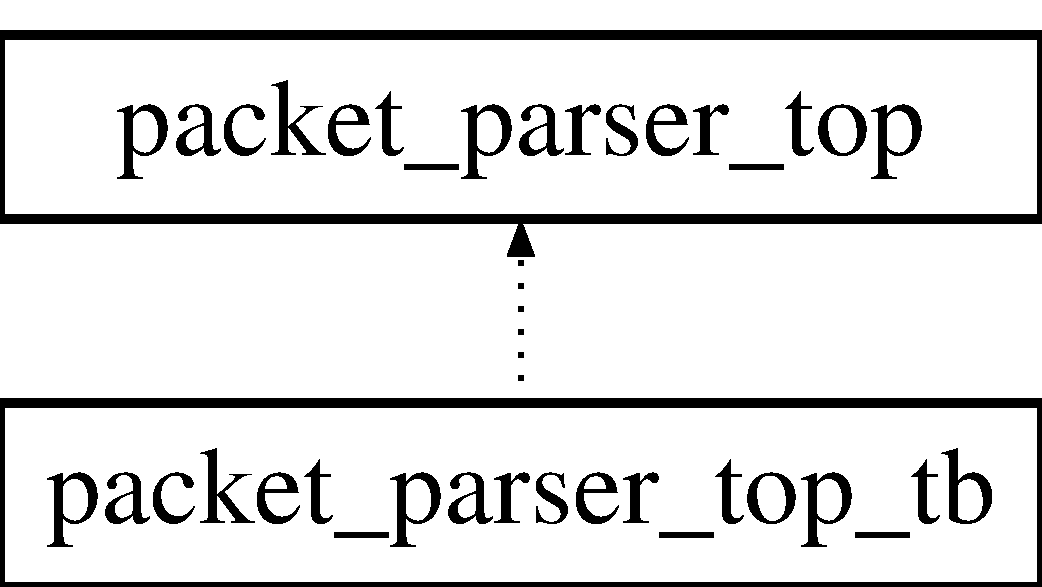
\includegraphics[height=2.000000cm]{enumpacket__parser__top}
\end{center}
\end{figure}


The documentation for this enum was generated from the following file\+:\begin{DoxyCompactItemize}
\item 
\mbox{\hyperlink{packet__parser__top_8v}{packet\+\_\+parser\+\_\+top.\+v}}\end{DoxyCompactItemize}

\hypertarget{enumpacket__parser__top__tb}{}\section{packet\+\_\+parser\+\_\+top\+\_\+tb Enum Reference}
\label{enumpacket__parser__top__tb}\index{packet\+\_\+parser\+\_\+top\+\_\+tb@{packet\+\_\+parser\+\_\+top\+\_\+tb}}
Inheritance diagram for packet\+\_\+parser\+\_\+top\+\_\+tb\+:\begin{figure}[H]
\begin{center}
\leavevmode
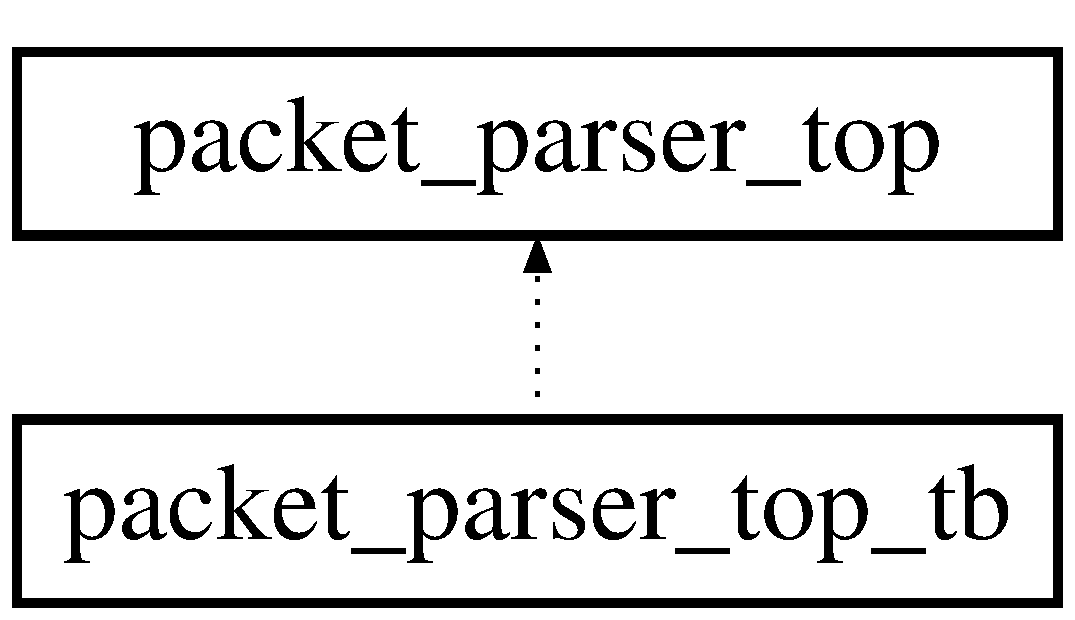
\includegraphics[height=2.000000cm]{enumpacket__parser__top__tb}
\end{center}
\end{figure}
\subsection*{Static Public Member Functions}
\begin{DoxyCompactItemize}
\item 
\mbox{\hyperlink{enumpacket__parser__top__tb_a17a60d01357f6cd3aa4f63a218b9eb5d}{P\+R\+O\+C\+E\+S\+S\+\_\+3}} Clk
\end{DoxyCompactItemize}
\subsection*{Public Attributes}
\begin{DoxyCompactItemize}
\item 
\mbox{\hyperlink{enumpacket__parser__top__tb_ad84a0b625ec2bdeadc59aa113a293bb6}{D\+A\+T\+A\+\_\+\+W\+I\+D\+TH}} \textquotesingle{}d64
\item 
\mbox{\hyperlink{enumpacket__parser__top__tb_a677494ad5b2330357e320a2cf124446d}{F\+I\+E\+L\+D\+\_\+\+N\+U\+M\+B\+ER}} 4
\item 
\mbox{\hyperlink{enumpacket__parser__top__tb_ae35d6a8982056bf50516d906dbb9e03a}{F\+I\+E\+L\+D\+\_\+\+S\+I\+Z\+E\+\_\+\+M\+AX}} 4
\item 
\mbox{[}(8 $\ast$F\+I\+E\+L\+D\+\_\+\+N\+U\+M\+B\+ER) -\/1\+:0 \mbox{\hyperlink{enumpacket__parser__top__tb_a60eeda70b6175d07efba4e010068e436}{F\+I\+E\+L\+D\+\_\+\+O\+F\+F\+S\+ET}} ) \{8 \textquotesingle{}d1 8 \textquotesingle{}d2 8 \textquotesingle{}d3 8 \textquotesingle{}d4\}
\item 
\mbox{[}(F\+I\+E\+L\+D\+\_\+\+S\+I\+Z\+E\+\_\+\+M\+AX $\ast$F\+I\+E\+L\+D\+\_\+\+N\+U\+M\+B\+ER $\ast$8) -\/1\+:0 \mbox{\hyperlink{enumpacket__parser__top__tb_aed76c3233df9cc658acb293145ac9acf}{F\+I\+E\+L\+D\+\_\+\+S\+I\+ZE}} ) \{32 \textquotesingle{}d1 32 \textquotesingle{}d2 32 \textquotesingle{}d3 32 \textquotesingle{}d4\}
\item 
\mbox{\hyperlink{enumpacket__parser__top__tb_a1af6e678e75aaa480ebe640a45e498fa}{Clk}} reg
\item 
\mbox{\hyperlink{enumpacket__parser__top__tb_a369a0a6fe6b71f3bf0fc3cd81147ea25}{Rst}} reg
\item 
\mbox{\hyperlink{enumpacket__parser__top__tb_a5be38cc71eddcc3aa3a4dcef49ca39b1}{In\+Bus\+\_\+\+Data\+Valid}} reg
\item 
\mbox{\hyperlink{enumpacket__parser__top__tb_a0ab0663aa4e7c8bea0e2d0745b8e1e08}{In\+Bus\+\_\+\+Data\+Sop}} reg
\item 
\mbox{\hyperlink{enumpacket__parser__top__tb_a58a9c1e3f5ddb0a8221edac4ad93c6f3}{In\+Bus\+\_\+\+Data\+Eop}} reg
\item 
\mbox{\hyperlink{enumpacket__parser__top__tb_a38d81d687bc91dee664724efd779a51b}{In\+Bus\+\_\+\+Mod}} reg\mbox{[} \$clog2\+D\+A\+T\+A\+\_\+\+W\+I\+D\+TH/8-\/1\+:0\mbox{]}
\item 
\mbox{\hyperlink{enumpacket__parser__top__tb_a6c2ee8e7409b36aa0ae95ddc49160f40}{In\+Bus\+\_\+\+Data}} reg\mbox{[}D\+A\+T\+A\+\_\+\+W\+I\+D\+TH-\/1\+:0\mbox{]}
\item 
\mbox{\hyperlink{enumpacket__parser__top__tb_a5dd0c370f9f3878f3cad8cebe29247e7}{Out\+Bus\+\_\+\+All\+Values\+\_\+\+Ready}} wire
\item 
\mbox{\hyperlink{enumpacket__parser__top__tb_a94de2bf629795d3141982ea31f81b022}{Out\+Bus\+\_\+\+Field\+\_\+muxed}} wire\mbox{[}F\+I\+E\+L\+D\+\_\+\+N\+U\+M\+B\+ER $\ast$F\+I\+E\+L\+D\+\_\+\+S\+I\+Z\+E\+\_\+\+M\+AX $\ast$8-\/1\+:0\mbox{]}
\item 
\mbox{\hyperlink{enumpacket__parser__top__tb_a8a933d6ad6c7c73fcd484ff507756e4d}{Out\+Bus\+\_\+\+Valid\+\_\+muxed}} wire\mbox{[}F\+I\+E\+L\+D\+\_\+\+N\+U\+M\+B\+ER-\/1\+:0\mbox{]}
\item 
\mbox{\hyperlink{enumpacket__parser__top__tb_ac4fa1b2e273138ab1b8386d1ac1dbc86}{error\+\_\+offset\+\_\+or\+\_\+size\+\_\+muxed}} wire\mbox{[}F\+I\+E\+L\+D\+\_\+\+N\+U\+M\+B\+ER-\/1\+:0\mbox{]}
\item 
\mbox{\hyperlink{enumpacket__parser__top__tb_a9228d47b399d20a20bed985c62c33268}{packet\+\_\+count}} reg\mbox{[} \$clog2\+M\+A\+X\+\_\+\+P\+K\+T\+S\+:0\mbox{]}
\item 
\mbox{\hyperlink{enumpacket__parser__top__tb_a0bf2ce1358b7e41a0b58a5b71b83274b}{packet\+\_\+size}} reg\mbox{[}15\+:0\mbox{]}
\item 
\mbox{\hyperlink{enumpacket__parser__top__tb_a3636615f10afd3d96c9b903a6ff17cab}{byte\+\_\+count}} reg\mbox{[}15\+:0\mbox{]}
\item 
\mbox{\hyperlink{enumpacket__parser__top__tb_a3edfc8715a60a7f03f7d12062c506e65}{field0}} reg\mbox{[}F\+I\+E\+L\+D\+\_\+\+S\+I\+Z\+E\+\_\+\+M\+AX $\ast$8-\/1\+:0\mbox{]}
\item 
\mbox{\hyperlink{enumpacket__parser__top__tb_a1c1ca0d195a8135b794463c2e1f2cf29}{field1}} reg\mbox{[}F\+I\+E\+L\+D\+\_\+\+S\+I\+Z\+E\+\_\+\+M\+AX $\ast$8-\/1\+:0\mbox{]}
\item 
\mbox{\hyperlink{enumpacket__parser__top__tb_ae5d6f0395c77f79679c1978a52202523}{field2}} reg\mbox{[}F\+I\+E\+L\+D\+\_\+\+S\+I\+Z\+E\+\_\+\+M\+AX $\ast$8-\/1\+:0\mbox{]}
\item 
\mbox{\hyperlink{enumpacket__parser__top__tb_a26ba4936dab335ee72f67aee1f08752d}{field3}} reg\mbox{[}F\+I\+E\+L\+D\+\_\+\+S\+I\+Z\+E\+\_\+\+M\+AX $\ast$8-\/1\+:0\mbox{]}
\item 
\mbox{\hyperlink{enumpacket__parser__top__tb_a0033d875cdf5314b3a76fd2d7ab13b2c}{queue\+\_\+out}} reg\mbox{[}F\+I\+E\+L\+D\+\_\+\+S\+I\+Z\+E\+\_\+\+M\+AX $\ast$F\+I\+E\+L\+D\+\_\+\+N\+U\+M\+B\+ER $\ast$8-\/1\+:0\mbox{]}
\item 
i \mbox{\hyperlink{enumpacket__parser__top__tb_a7123921cf22dcde880af6f141d7f186d}{packet\+\_\+parser\+\_\+top}}
\item 
\mbox{\hyperlink{enumpacket__parser__top__tb_a0feaee318fc79d5645a7a497966d79a2}{state}} reg\mbox{[}2\+:0\mbox{]}
\item 
\mbox{\hyperlink{enumpacket__parser__top__tb_a77f10db5d1edf2cbbf2ea75626bc130e}{I\+D\+LE}} 0
\item 
\mbox{\hyperlink{enumpacket__parser__top__tb_acc8439edf27c04ea18e30cbd0b85e4d7}{T\+X\+F\+R\+\_\+\+P\+KT}} 1
\item 
\mbox{\hyperlink{enumpacket__parser__top__tb_a12e0d38624187f2a91f99b60297754c2}{Out\+Bus\+\_\+\+All\+Values\+\_\+\+Ready\+\_\+d1}} reg
\item 
\mbox{\hyperlink{enumpacket__parser__top__tb_ae4b2da01c8aacb18bea197efcdb230f0}{all\+\_\+fields\+\_\+ready}} wire
\item 
\mbox{\hyperlink{enumpacket__parser__top__tb_afcfae2318d3fa2f468b7a09bb72a0345}{all\+\_\+fields\+\_\+ready\+\_\+d1}} reg
\item 
\mbox{\hyperlink{enumpacket__parser__top__tb_af1832ebe93b9257253409a07fb3c8a48}{wr\+\_\+addr}} reg\mbox{[}9\+:0\mbox{]}
\item 
\mbox{\hyperlink{enumpacket__parser__top__tb_a31ec51cb3369def58c9a65744ddbfa9a}{rd\+\_\+addr}} reg\mbox{[}9\+:0\mbox{]}
\item 
\mbox{\hyperlink{enumpacket__parser__top__tb_ad3a4f0399068428438a4d1280e7547d4}{push\+\_\+queue}} wire
\end{DoxyCompactItemize}


\subsection{Member Function Documentation}
\mbox{\Hypertarget{enumpacket__parser__top__tb_a17a60d01357f6cd3aa4f63a218b9eb5d}\label{enumpacket__parser__top__tb_a17a60d01357f6cd3aa4f63a218b9eb5d}} 
\index{packet\+\_\+parser\+\_\+top\+\_\+tb@{packet\+\_\+parser\+\_\+top\+\_\+tb}!P\+R\+O\+C\+E\+S\+S\+\_\+3@{P\+R\+O\+C\+E\+S\+S\+\_\+3}}
\index{P\+R\+O\+C\+E\+S\+S\+\_\+3@{P\+R\+O\+C\+E\+S\+S\+\_\+3}!packet\+\_\+parser\+\_\+top\+\_\+tb@{packet\+\_\+parser\+\_\+top\+\_\+tb}}
\subsubsection{\texorpdfstring{P\+R\+O\+C\+E\+S\+S\+\_\+3()}{PROCESS\_3()}}
{\footnotesize\ttfamily \hspace{0.3cm}}



\subsection{Member Data Documentation}
\mbox{\Hypertarget{enumpacket__parser__top__tb_ad84a0b625ec2bdeadc59aa113a293bb6}\label{enumpacket__parser__top__tb_ad84a0b625ec2bdeadc59aa113a293bb6}} 
\index{packet\+\_\+parser\+\_\+top\+\_\+tb@{packet\+\_\+parser\+\_\+top\+\_\+tb}!D\+A\+T\+A\+\_\+\+W\+I\+D\+TH@{D\+A\+T\+A\+\_\+\+W\+I\+D\+TH}}
\index{D\+A\+T\+A\+\_\+\+W\+I\+D\+TH@{D\+A\+T\+A\+\_\+\+W\+I\+D\+TH}!packet\+\_\+parser\+\_\+top\+\_\+tb@{packet\+\_\+parser\+\_\+top\+\_\+tb}}
\subsubsection{\texorpdfstring{D\+A\+T\+A\+\_\+\+W\+I\+D\+TH}{DATA\_WIDTH}}
{\footnotesize\ttfamily \mbox{\hyperlink{enumpacket__parser__top__tb_ad84a0b625ec2bdeadc59aa113a293bb6}{D\+A\+T\+A\+\_\+\+W\+I\+D\+TH}} {\bfseries \textcolor{vhdlchar}{ }} \hspace{0.3cm}}

\mbox{\Hypertarget{enumpacket__parser__top__tb_a677494ad5b2330357e320a2cf124446d}\label{enumpacket__parser__top__tb_a677494ad5b2330357e320a2cf124446d}} 
\index{packet\+\_\+parser\+\_\+top\+\_\+tb@{packet\+\_\+parser\+\_\+top\+\_\+tb}!F\+I\+E\+L\+D\+\_\+\+N\+U\+M\+B\+ER@{F\+I\+E\+L\+D\+\_\+\+N\+U\+M\+B\+ER}}
\index{F\+I\+E\+L\+D\+\_\+\+N\+U\+M\+B\+ER@{F\+I\+E\+L\+D\+\_\+\+N\+U\+M\+B\+ER}!packet\+\_\+parser\+\_\+top\+\_\+tb@{packet\+\_\+parser\+\_\+top\+\_\+tb}}
\subsubsection{\texorpdfstring{F\+I\+E\+L\+D\+\_\+\+N\+U\+M\+B\+ER}{FIELD\_NUMBER}}
{\footnotesize\ttfamily \mbox{\hyperlink{enumpacket__parser__top__tb_a677494ad5b2330357e320a2cf124446d}{F\+I\+E\+L\+D\+\_\+\+N\+U\+M\+B\+ER}} {\bfseries \textcolor{vhdlchar}{ }} \hspace{0.3cm}}

\mbox{\Hypertarget{enumpacket__parser__top__tb_ae35d6a8982056bf50516d906dbb9e03a}\label{enumpacket__parser__top__tb_ae35d6a8982056bf50516d906dbb9e03a}} 
\index{packet\+\_\+parser\+\_\+top\+\_\+tb@{packet\+\_\+parser\+\_\+top\+\_\+tb}!F\+I\+E\+L\+D\+\_\+\+S\+I\+Z\+E\+\_\+\+M\+AX@{F\+I\+E\+L\+D\+\_\+\+S\+I\+Z\+E\+\_\+\+M\+AX}}
\index{F\+I\+E\+L\+D\+\_\+\+S\+I\+Z\+E\+\_\+\+M\+AX@{F\+I\+E\+L\+D\+\_\+\+S\+I\+Z\+E\+\_\+\+M\+AX}!packet\+\_\+parser\+\_\+top\+\_\+tb@{packet\+\_\+parser\+\_\+top\+\_\+tb}}
\subsubsection{\texorpdfstring{F\+I\+E\+L\+D\+\_\+\+S\+I\+Z\+E\+\_\+\+M\+AX}{FIELD\_SIZE\_MAX}}
{\footnotesize\ttfamily \mbox{\hyperlink{enumpacket__parser__top__tb_ae35d6a8982056bf50516d906dbb9e03a}{F\+I\+E\+L\+D\+\_\+\+S\+I\+Z\+E\+\_\+\+M\+AX}} {\bfseries \textcolor{vhdlchar}{ }} \hspace{0.3cm}}

\mbox{\Hypertarget{enumpacket__parser__top__tb_a60eeda70b6175d07efba4e010068e436}\label{enumpacket__parser__top__tb_a60eeda70b6175d07efba4e010068e436}} 
\index{packet\+\_\+parser\+\_\+top\+\_\+tb@{packet\+\_\+parser\+\_\+top\+\_\+tb}!F\+I\+E\+L\+D\+\_\+\+O\+F\+F\+S\+ET@{F\+I\+E\+L\+D\+\_\+\+O\+F\+F\+S\+ET}}
\index{F\+I\+E\+L\+D\+\_\+\+O\+F\+F\+S\+ET@{F\+I\+E\+L\+D\+\_\+\+O\+F\+F\+S\+ET}!packet\+\_\+parser\+\_\+top\+\_\+tb@{packet\+\_\+parser\+\_\+top\+\_\+tb}}
\subsubsection{\texorpdfstring{F\+I\+E\+L\+D\+\_\+\+O\+F\+F\+S\+ET}{FIELD\_OFFSET}}
{\footnotesize\ttfamily \mbox{\hyperlink{enumpacket__parser__top__tb_a60eeda70b6175d07efba4e010068e436}{F\+I\+E\+L\+D\+\_\+\+O\+F\+F\+S\+ET}} {\bfseries \textcolor{vhdlchar}{\mbox{[}}\textcolor{vhdlchar}{ }\textcolor{vhdlchar}{(}\textcolor{vhdlchar}{ } \textcolor{vhdldigit}{8} \textcolor{vhdlchar}{ }\textcolor{vhdlchar}{$\ast$}{\bfseries \mbox{\hyperlink{enumpacket__parser__top__tb_a677494ad5b2330357e320a2cf124446d}{F\+I\+E\+L\+D\+\_\+\+N\+U\+M\+B\+ER}}} \textcolor{vhdlchar}{ }\textcolor{vhdlchar}{)}\textcolor{vhdlchar}{ }\textcolor{vhdlchar}{ }\textcolor{vhdlchar}{-\/} \textcolor{vhdldigit}{1} \textcolor{vhdlchar}{ }\textcolor{vhdlchar}{\+:}\textcolor{vhdlchar}{ } \textcolor{vhdldigit}{0} \textcolor{vhdlchar}{ }} \hspace{0.3cm}}

\mbox{\Hypertarget{enumpacket__parser__top__tb_aed76c3233df9cc658acb293145ac9acf}\label{enumpacket__parser__top__tb_aed76c3233df9cc658acb293145ac9acf}} 
\index{packet\+\_\+parser\+\_\+top\+\_\+tb@{packet\+\_\+parser\+\_\+top\+\_\+tb}!F\+I\+E\+L\+D\+\_\+\+S\+I\+ZE@{F\+I\+E\+L\+D\+\_\+\+S\+I\+ZE}}
\index{F\+I\+E\+L\+D\+\_\+\+S\+I\+ZE@{F\+I\+E\+L\+D\+\_\+\+S\+I\+ZE}!packet\+\_\+parser\+\_\+top\+\_\+tb@{packet\+\_\+parser\+\_\+top\+\_\+tb}}
\subsubsection{\texorpdfstring{F\+I\+E\+L\+D\+\_\+\+S\+I\+ZE}{FIELD\_SIZE}}
{\footnotesize\ttfamily \mbox{\hyperlink{enumpacket__parser__top__tb_aed76c3233df9cc658acb293145ac9acf}{F\+I\+E\+L\+D\+\_\+\+S\+I\+ZE}} {\bfseries \textcolor{vhdlchar}{\mbox{[}}\textcolor{vhdlchar}{ }\textcolor{vhdlchar}{(}\textcolor{vhdlchar}{ }{\bfseries \mbox{\hyperlink{enumpacket__parser__top__tb_ae35d6a8982056bf50516d906dbb9e03a}{F\+I\+E\+L\+D\+\_\+\+S\+I\+Z\+E\+\_\+\+M\+AX}}} \textcolor{vhdlchar}{ }\textcolor{vhdlchar}{$\ast$}{\bfseries \mbox{\hyperlink{enumpacket__parser__top__tb_a677494ad5b2330357e320a2cf124446d}{F\+I\+E\+L\+D\+\_\+\+N\+U\+M\+B\+ER}}} \textcolor{vhdlchar}{ }\textcolor{vhdlchar}{$\ast$} \textcolor{vhdldigit}{8} \textcolor{vhdlchar}{ }\textcolor{vhdlchar}{)}\textcolor{vhdlchar}{ }\textcolor{vhdlchar}{ }\textcolor{vhdlchar}{-\/} \textcolor{vhdldigit}{1} \textcolor{vhdlchar}{ }\textcolor{vhdlchar}{\+:}\textcolor{vhdlchar}{ } \textcolor{vhdldigit}{0} \textcolor{vhdlchar}{ }} \hspace{0.3cm}}

\mbox{\Hypertarget{enumpacket__parser__top__tb_a1af6e678e75aaa480ebe640a45e498fa}\label{enumpacket__parser__top__tb_a1af6e678e75aaa480ebe640a45e498fa}} 
\index{packet\+\_\+parser\+\_\+top\+\_\+tb@{packet\+\_\+parser\+\_\+top\+\_\+tb}!Clk@{Clk}}
\index{Clk@{Clk}!packet\+\_\+parser\+\_\+top\+\_\+tb@{packet\+\_\+parser\+\_\+top\+\_\+tb}}
\subsubsection{\texorpdfstring{Clk}{Clk}}
{\footnotesize\ttfamily \mbox{\hyperlink{enumpacket__parser__top__tb_a1af6e678e75aaa480ebe640a45e498fa}{Clk}} {\bfseries \textcolor{vhdlchar}{ }} \hspace{0.3cm}}

\mbox{\Hypertarget{enumpacket__parser__top__tb_a369a0a6fe6b71f3bf0fc3cd81147ea25}\label{enumpacket__parser__top__tb_a369a0a6fe6b71f3bf0fc3cd81147ea25}} 
\index{packet\+\_\+parser\+\_\+top\+\_\+tb@{packet\+\_\+parser\+\_\+top\+\_\+tb}!Rst@{Rst}}
\index{Rst@{Rst}!packet\+\_\+parser\+\_\+top\+\_\+tb@{packet\+\_\+parser\+\_\+top\+\_\+tb}}
\subsubsection{\texorpdfstring{Rst}{Rst}}
{\footnotesize\ttfamily \mbox{\hyperlink{enumpacket__parser__top__tb_a369a0a6fe6b71f3bf0fc3cd81147ea25}{Rst}} {\bfseries \textcolor{vhdlchar}{ }} \hspace{0.3cm}}

\mbox{\Hypertarget{enumpacket__parser__top__tb_a5be38cc71eddcc3aa3a4dcef49ca39b1}\label{enumpacket__parser__top__tb_a5be38cc71eddcc3aa3a4dcef49ca39b1}} 
\index{packet\+\_\+parser\+\_\+top\+\_\+tb@{packet\+\_\+parser\+\_\+top\+\_\+tb}!In\+Bus\+\_\+\+Data\+Valid@{In\+Bus\+\_\+\+Data\+Valid}}
\index{In\+Bus\+\_\+\+Data\+Valid@{In\+Bus\+\_\+\+Data\+Valid}!packet\+\_\+parser\+\_\+top\+\_\+tb@{packet\+\_\+parser\+\_\+top\+\_\+tb}}
\subsubsection{\texorpdfstring{In\+Bus\+\_\+\+Data\+Valid}{InBus\_DataValid}}
{\footnotesize\ttfamily \mbox{\hyperlink{enumpacket__parser__top__tb_a5be38cc71eddcc3aa3a4dcef49ca39b1}{In\+Bus\+\_\+\+Data\+Valid}} {\bfseries \textcolor{vhdlchar}{ }} \hspace{0.3cm}}

\mbox{\Hypertarget{enumpacket__parser__top__tb_a0ab0663aa4e7c8bea0e2d0745b8e1e08}\label{enumpacket__parser__top__tb_a0ab0663aa4e7c8bea0e2d0745b8e1e08}} 
\index{packet\+\_\+parser\+\_\+top\+\_\+tb@{packet\+\_\+parser\+\_\+top\+\_\+tb}!In\+Bus\+\_\+\+Data\+Sop@{In\+Bus\+\_\+\+Data\+Sop}}
\index{In\+Bus\+\_\+\+Data\+Sop@{In\+Bus\+\_\+\+Data\+Sop}!packet\+\_\+parser\+\_\+top\+\_\+tb@{packet\+\_\+parser\+\_\+top\+\_\+tb}}
\subsubsection{\texorpdfstring{In\+Bus\+\_\+\+Data\+Sop}{InBus\_DataSop}}
{\footnotesize\ttfamily \mbox{\hyperlink{enumpacket__parser__top__tb_a0ab0663aa4e7c8bea0e2d0745b8e1e08}{In\+Bus\+\_\+\+Data\+Sop}} {\bfseries \textcolor{vhdlchar}{ }} \hspace{0.3cm}}

\mbox{\Hypertarget{enumpacket__parser__top__tb_a58a9c1e3f5ddb0a8221edac4ad93c6f3}\label{enumpacket__parser__top__tb_a58a9c1e3f5ddb0a8221edac4ad93c6f3}} 
\index{packet\+\_\+parser\+\_\+top\+\_\+tb@{packet\+\_\+parser\+\_\+top\+\_\+tb}!In\+Bus\+\_\+\+Data\+Eop@{In\+Bus\+\_\+\+Data\+Eop}}
\index{In\+Bus\+\_\+\+Data\+Eop@{In\+Bus\+\_\+\+Data\+Eop}!packet\+\_\+parser\+\_\+top\+\_\+tb@{packet\+\_\+parser\+\_\+top\+\_\+tb}}
\subsubsection{\texorpdfstring{In\+Bus\+\_\+\+Data\+Eop}{InBus\_DataEop}}
{\footnotesize\ttfamily \mbox{\hyperlink{enumpacket__parser__top__tb_a58a9c1e3f5ddb0a8221edac4ad93c6f3}{In\+Bus\+\_\+\+Data\+Eop}} {\bfseries \textcolor{vhdlchar}{ }} \hspace{0.3cm}}

\mbox{\Hypertarget{enumpacket__parser__top__tb_a38d81d687bc91dee664724efd779a51b}\label{enumpacket__parser__top__tb_a38d81d687bc91dee664724efd779a51b}} 
\index{packet\+\_\+parser\+\_\+top\+\_\+tb@{packet\+\_\+parser\+\_\+top\+\_\+tb}!In\+Bus\+\_\+\+Mod@{In\+Bus\+\_\+\+Mod}}
\index{In\+Bus\+\_\+\+Mod@{In\+Bus\+\_\+\+Mod}!packet\+\_\+parser\+\_\+top\+\_\+tb@{packet\+\_\+parser\+\_\+top\+\_\+tb}}
\subsubsection{\texorpdfstring{In\+Bus\+\_\+\+Mod}{InBus\_Mod}}
{\footnotesize\ttfamily \mbox{\hyperlink{enumpacket__parser__top__tb_a38d81d687bc91dee664724efd779a51b}{In\+Bus\+\_\+\+Mod}} {\bfseries \textcolor{vhdlchar}{ }} \hspace{0.3cm}}

\mbox{\Hypertarget{enumpacket__parser__top__tb_a6c2ee8e7409b36aa0ae95ddc49160f40}\label{enumpacket__parser__top__tb_a6c2ee8e7409b36aa0ae95ddc49160f40}} 
\index{packet\+\_\+parser\+\_\+top\+\_\+tb@{packet\+\_\+parser\+\_\+top\+\_\+tb}!In\+Bus\+\_\+\+Data@{In\+Bus\+\_\+\+Data}}
\index{In\+Bus\+\_\+\+Data@{In\+Bus\+\_\+\+Data}!packet\+\_\+parser\+\_\+top\+\_\+tb@{packet\+\_\+parser\+\_\+top\+\_\+tb}}
\subsubsection{\texorpdfstring{In\+Bus\+\_\+\+Data}{InBus\_Data}}
{\footnotesize\ttfamily \mbox{\hyperlink{enumpacket__parser__top__tb_a6c2ee8e7409b36aa0ae95ddc49160f40}{In\+Bus\+\_\+\+Data}} {\bfseries \textcolor{vhdlchar}{ }} \hspace{0.3cm}}

\mbox{\Hypertarget{enumpacket__parser__top__tb_a5dd0c370f9f3878f3cad8cebe29247e7}\label{enumpacket__parser__top__tb_a5dd0c370f9f3878f3cad8cebe29247e7}} 
\index{packet\+\_\+parser\+\_\+top\+\_\+tb@{packet\+\_\+parser\+\_\+top\+\_\+tb}!Out\+Bus\+\_\+\+All\+Values\+\_\+\+Ready@{Out\+Bus\+\_\+\+All\+Values\+\_\+\+Ready}}
\index{Out\+Bus\+\_\+\+All\+Values\+\_\+\+Ready@{Out\+Bus\+\_\+\+All\+Values\+\_\+\+Ready}!packet\+\_\+parser\+\_\+top\+\_\+tb@{packet\+\_\+parser\+\_\+top\+\_\+tb}}
\subsubsection{\texorpdfstring{Out\+Bus\+\_\+\+All\+Values\+\_\+\+Ready}{OutBus\_AllValues\_Ready}}
{\footnotesize\ttfamily \mbox{\hyperlink{enumpacket__parser__top__tb_a5dd0c370f9f3878f3cad8cebe29247e7}{Out\+Bus\+\_\+\+All\+Values\+\_\+\+Ready}} {\bfseries \textcolor{vhdlchar}{ }} \hspace{0.3cm}}

\mbox{\Hypertarget{enumpacket__parser__top__tb_a94de2bf629795d3141982ea31f81b022}\label{enumpacket__parser__top__tb_a94de2bf629795d3141982ea31f81b022}} 
\index{packet\+\_\+parser\+\_\+top\+\_\+tb@{packet\+\_\+parser\+\_\+top\+\_\+tb}!Out\+Bus\+\_\+\+Field\+\_\+muxed@{Out\+Bus\+\_\+\+Field\+\_\+muxed}}
\index{Out\+Bus\+\_\+\+Field\+\_\+muxed@{Out\+Bus\+\_\+\+Field\+\_\+muxed}!packet\+\_\+parser\+\_\+top\+\_\+tb@{packet\+\_\+parser\+\_\+top\+\_\+tb}}
\subsubsection{\texorpdfstring{Out\+Bus\+\_\+\+Field\+\_\+muxed}{OutBus\_Field\_muxed}}
{\footnotesize\ttfamily \mbox{\hyperlink{enumpacket__parser__top__tb_a94de2bf629795d3141982ea31f81b022}{Out\+Bus\+\_\+\+Field\+\_\+muxed}} {\bfseries \textcolor{vhdlchar}{ }} \hspace{0.3cm}}

\mbox{\Hypertarget{enumpacket__parser__top__tb_a8a933d6ad6c7c73fcd484ff507756e4d}\label{enumpacket__parser__top__tb_a8a933d6ad6c7c73fcd484ff507756e4d}} 
\index{packet\+\_\+parser\+\_\+top\+\_\+tb@{packet\+\_\+parser\+\_\+top\+\_\+tb}!Out\+Bus\+\_\+\+Valid\+\_\+muxed@{Out\+Bus\+\_\+\+Valid\+\_\+muxed}}
\index{Out\+Bus\+\_\+\+Valid\+\_\+muxed@{Out\+Bus\+\_\+\+Valid\+\_\+muxed}!packet\+\_\+parser\+\_\+top\+\_\+tb@{packet\+\_\+parser\+\_\+top\+\_\+tb}}
\subsubsection{\texorpdfstring{Out\+Bus\+\_\+\+Valid\+\_\+muxed}{OutBus\_Valid\_muxed}}
{\footnotesize\ttfamily \mbox{\hyperlink{enumpacket__parser__top__tb_a8a933d6ad6c7c73fcd484ff507756e4d}{Out\+Bus\+\_\+\+Valid\+\_\+muxed}} {\bfseries \textcolor{vhdlchar}{ }} \hspace{0.3cm}}

\mbox{\Hypertarget{enumpacket__parser__top__tb_ac4fa1b2e273138ab1b8386d1ac1dbc86}\label{enumpacket__parser__top__tb_ac4fa1b2e273138ab1b8386d1ac1dbc86}} 
\index{packet\+\_\+parser\+\_\+top\+\_\+tb@{packet\+\_\+parser\+\_\+top\+\_\+tb}!error\+\_\+offset\+\_\+or\+\_\+size\+\_\+muxed@{error\+\_\+offset\+\_\+or\+\_\+size\+\_\+muxed}}
\index{error\+\_\+offset\+\_\+or\+\_\+size\+\_\+muxed@{error\+\_\+offset\+\_\+or\+\_\+size\+\_\+muxed}!packet\+\_\+parser\+\_\+top\+\_\+tb@{packet\+\_\+parser\+\_\+top\+\_\+tb}}
\subsubsection{\texorpdfstring{error\+\_\+offset\+\_\+or\+\_\+size\+\_\+muxed}{error\_offset\_or\_size\_muxed}}
{\footnotesize\ttfamily \mbox{\hyperlink{enumpacket__parser__top__tb_ac4fa1b2e273138ab1b8386d1ac1dbc86}{error\+\_\+offset\+\_\+or\+\_\+size\+\_\+muxed}} {\bfseries \textcolor{vhdlchar}{ }} \hspace{0.3cm}}

\mbox{\Hypertarget{enumpacket__parser__top__tb_a9228d47b399d20a20bed985c62c33268}\label{enumpacket__parser__top__tb_a9228d47b399d20a20bed985c62c33268}} 
\index{packet\+\_\+parser\+\_\+top\+\_\+tb@{packet\+\_\+parser\+\_\+top\+\_\+tb}!packet\+\_\+count@{packet\+\_\+count}}
\index{packet\+\_\+count@{packet\+\_\+count}!packet\+\_\+parser\+\_\+top\+\_\+tb@{packet\+\_\+parser\+\_\+top\+\_\+tb}}
\subsubsection{\texorpdfstring{packet\+\_\+count}{packet\_count}}
{\footnotesize\ttfamily \mbox{\hyperlink{enumpacket__parser__top__tb_a9228d47b399d20a20bed985c62c33268}{packet\+\_\+count}} {\bfseries \textcolor{vhdlchar}{ }} \hspace{0.3cm}}

\mbox{\Hypertarget{enumpacket__parser__top__tb_a0bf2ce1358b7e41a0b58a5b71b83274b}\label{enumpacket__parser__top__tb_a0bf2ce1358b7e41a0b58a5b71b83274b}} 
\index{packet\+\_\+parser\+\_\+top\+\_\+tb@{packet\+\_\+parser\+\_\+top\+\_\+tb}!packet\+\_\+size@{packet\+\_\+size}}
\index{packet\+\_\+size@{packet\+\_\+size}!packet\+\_\+parser\+\_\+top\+\_\+tb@{packet\+\_\+parser\+\_\+top\+\_\+tb}}
\subsubsection{\texorpdfstring{packet\+\_\+size}{packet\_size}}
{\footnotesize\ttfamily \mbox{\hyperlink{enumpacket__parser__top__tb_a0bf2ce1358b7e41a0b58a5b71b83274b}{packet\+\_\+size}} {\bfseries \textcolor{vhdlchar}{ }} \hspace{0.3cm}}

\mbox{\Hypertarget{enumpacket__parser__top__tb_a3636615f10afd3d96c9b903a6ff17cab}\label{enumpacket__parser__top__tb_a3636615f10afd3d96c9b903a6ff17cab}} 
\index{packet\+\_\+parser\+\_\+top\+\_\+tb@{packet\+\_\+parser\+\_\+top\+\_\+tb}!byte\+\_\+count@{byte\+\_\+count}}
\index{byte\+\_\+count@{byte\+\_\+count}!packet\+\_\+parser\+\_\+top\+\_\+tb@{packet\+\_\+parser\+\_\+top\+\_\+tb}}
\subsubsection{\texorpdfstring{byte\+\_\+count}{byte\_count}}
{\footnotesize\ttfamily \mbox{\hyperlink{enumpacket__parser__top__tb_a3636615f10afd3d96c9b903a6ff17cab}{byte\+\_\+count}} {\bfseries \textcolor{vhdlchar}{ }} \hspace{0.3cm}}

\mbox{\Hypertarget{enumpacket__parser__top__tb_a3edfc8715a60a7f03f7d12062c506e65}\label{enumpacket__parser__top__tb_a3edfc8715a60a7f03f7d12062c506e65}} 
\index{packet\+\_\+parser\+\_\+top\+\_\+tb@{packet\+\_\+parser\+\_\+top\+\_\+tb}!field0@{field0}}
\index{field0@{field0}!packet\+\_\+parser\+\_\+top\+\_\+tb@{packet\+\_\+parser\+\_\+top\+\_\+tb}}
\subsubsection{\texorpdfstring{field0}{field0}}
{\footnotesize\ttfamily \mbox{\hyperlink{enumpacket__parser__top__tb_a3edfc8715a60a7f03f7d12062c506e65}{field0}} {\bfseries \textcolor{vhdlchar}{ }} \hspace{0.3cm}}

\mbox{\Hypertarget{enumpacket__parser__top__tb_a1c1ca0d195a8135b794463c2e1f2cf29}\label{enumpacket__parser__top__tb_a1c1ca0d195a8135b794463c2e1f2cf29}} 
\index{packet\+\_\+parser\+\_\+top\+\_\+tb@{packet\+\_\+parser\+\_\+top\+\_\+tb}!field1@{field1}}
\index{field1@{field1}!packet\+\_\+parser\+\_\+top\+\_\+tb@{packet\+\_\+parser\+\_\+top\+\_\+tb}}
\subsubsection{\texorpdfstring{field1}{field1}}
{\footnotesize\ttfamily \mbox{\hyperlink{enumpacket__parser__top__tb_a1c1ca0d195a8135b794463c2e1f2cf29}{field1}} {\bfseries \textcolor{vhdlchar}{ }} \hspace{0.3cm}}

\mbox{\Hypertarget{enumpacket__parser__top__tb_ae5d6f0395c77f79679c1978a52202523}\label{enumpacket__parser__top__tb_ae5d6f0395c77f79679c1978a52202523}} 
\index{packet\+\_\+parser\+\_\+top\+\_\+tb@{packet\+\_\+parser\+\_\+top\+\_\+tb}!field2@{field2}}
\index{field2@{field2}!packet\+\_\+parser\+\_\+top\+\_\+tb@{packet\+\_\+parser\+\_\+top\+\_\+tb}}
\subsubsection{\texorpdfstring{field2}{field2}}
{\footnotesize\ttfamily \mbox{\hyperlink{enumpacket__parser__top__tb_ae5d6f0395c77f79679c1978a52202523}{field2}} {\bfseries \textcolor{vhdlchar}{ }} \hspace{0.3cm}}

\mbox{\Hypertarget{enumpacket__parser__top__tb_a26ba4936dab335ee72f67aee1f08752d}\label{enumpacket__parser__top__tb_a26ba4936dab335ee72f67aee1f08752d}} 
\index{packet\+\_\+parser\+\_\+top\+\_\+tb@{packet\+\_\+parser\+\_\+top\+\_\+tb}!field3@{field3}}
\index{field3@{field3}!packet\+\_\+parser\+\_\+top\+\_\+tb@{packet\+\_\+parser\+\_\+top\+\_\+tb}}
\subsubsection{\texorpdfstring{field3}{field3}}
{\footnotesize\ttfamily \mbox{\hyperlink{enumpacket__parser__top__tb_a26ba4936dab335ee72f67aee1f08752d}{field3}} {\bfseries \textcolor{vhdlchar}{ }} \hspace{0.3cm}}

\mbox{\Hypertarget{enumpacket__parser__top__tb_a0033d875cdf5314b3a76fd2d7ab13b2c}\label{enumpacket__parser__top__tb_a0033d875cdf5314b3a76fd2d7ab13b2c}} 
\index{packet\+\_\+parser\+\_\+top\+\_\+tb@{packet\+\_\+parser\+\_\+top\+\_\+tb}!queue\+\_\+out@{queue\+\_\+out}}
\index{queue\+\_\+out@{queue\+\_\+out}!packet\+\_\+parser\+\_\+top\+\_\+tb@{packet\+\_\+parser\+\_\+top\+\_\+tb}}
\subsubsection{\texorpdfstring{queue\+\_\+out}{queue\_out}}
{\footnotesize\ttfamily \mbox{\hyperlink{enumpacket__parser__top__tb_a0033d875cdf5314b3a76fd2d7ab13b2c}{queue\+\_\+out}} {\bfseries \textcolor{vhdlchar}{ }} \hspace{0.3cm}}

\mbox{\Hypertarget{enumpacket__parser__top__tb_a0feaee318fc79d5645a7a497966d79a2}\label{enumpacket__parser__top__tb_a0feaee318fc79d5645a7a497966d79a2}} 
\index{packet\+\_\+parser\+\_\+top\+\_\+tb@{packet\+\_\+parser\+\_\+top\+\_\+tb}!state@{state}}
\index{state@{state}!packet\+\_\+parser\+\_\+top\+\_\+tb@{packet\+\_\+parser\+\_\+top\+\_\+tb}}
\subsubsection{\texorpdfstring{state}{state}}
{\footnotesize\ttfamily \mbox{\hyperlink{enumpacket__parser__top__tb_a0feaee318fc79d5645a7a497966d79a2}{state}} {\bfseries \textcolor{vhdlchar}{ }} \hspace{0.3cm}}

\mbox{\Hypertarget{enumpacket__parser__top__tb_a77f10db5d1edf2cbbf2ea75626bc130e}\label{enumpacket__parser__top__tb_a77f10db5d1edf2cbbf2ea75626bc130e}} 
\index{packet\+\_\+parser\+\_\+top\+\_\+tb@{packet\+\_\+parser\+\_\+top\+\_\+tb}!I\+D\+LE@{I\+D\+LE}}
\index{I\+D\+LE@{I\+D\+LE}!packet\+\_\+parser\+\_\+top\+\_\+tb@{packet\+\_\+parser\+\_\+top\+\_\+tb}}
\subsubsection{\texorpdfstring{I\+D\+LE}{IDLE}}
{\footnotesize\ttfamily \mbox{\hyperlink{enumpacket__parser__top__tb_a77f10db5d1edf2cbbf2ea75626bc130e}{I\+D\+LE}} {\bfseries \textcolor{vhdlchar}{ }} \hspace{0.3cm}}

\mbox{\Hypertarget{enumpacket__parser__top__tb_acc8439edf27c04ea18e30cbd0b85e4d7}\label{enumpacket__parser__top__tb_acc8439edf27c04ea18e30cbd0b85e4d7}} 
\index{packet\+\_\+parser\+\_\+top\+\_\+tb@{packet\+\_\+parser\+\_\+top\+\_\+tb}!T\+X\+F\+R\+\_\+\+P\+KT@{T\+X\+F\+R\+\_\+\+P\+KT}}
\index{T\+X\+F\+R\+\_\+\+P\+KT@{T\+X\+F\+R\+\_\+\+P\+KT}!packet\+\_\+parser\+\_\+top\+\_\+tb@{packet\+\_\+parser\+\_\+top\+\_\+tb}}
\subsubsection{\texorpdfstring{T\+X\+F\+R\+\_\+\+P\+KT}{TXFR\_PKT}}
{\footnotesize\ttfamily \mbox{\hyperlink{enumpacket__parser__top__tb_acc8439edf27c04ea18e30cbd0b85e4d7}{T\+X\+F\+R\+\_\+\+P\+KT}} {\bfseries \textcolor{vhdlchar}{ }} \hspace{0.3cm}}

\mbox{\Hypertarget{enumpacket__parser__top__tb_a12e0d38624187f2a91f99b60297754c2}\label{enumpacket__parser__top__tb_a12e0d38624187f2a91f99b60297754c2}} 
\index{packet\+\_\+parser\+\_\+top\+\_\+tb@{packet\+\_\+parser\+\_\+top\+\_\+tb}!Out\+Bus\+\_\+\+All\+Values\+\_\+\+Ready\+\_\+d1@{Out\+Bus\+\_\+\+All\+Values\+\_\+\+Ready\+\_\+d1}}
\index{Out\+Bus\+\_\+\+All\+Values\+\_\+\+Ready\+\_\+d1@{Out\+Bus\+\_\+\+All\+Values\+\_\+\+Ready\+\_\+d1}!packet\+\_\+parser\+\_\+top\+\_\+tb@{packet\+\_\+parser\+\_\+top\+\_\+tb}}
\subsubsection{\texorpdfstring{Out\+Bus\+\_\+\+All\+Values\+\_\+\+Ready\+\_\+d1}{OutBus\_AllValues\_Ready\_d1}}
{\footnotesize\ttfamily \mbox{\hyperlink{enumpacket__parser__top__tb_a12e0d38624187f2a91f99b60297754c2}{Out\+Bus\+\_\+\+All\+Values\+\_\+\+Ready\+\_\+d1}} {\bfseries \textcolor{vhdlchar}{ }} \hspace{0.3cm}}

\mbox{\Hypertarget{enumpacket__parser__top__tb_ae4b2da01c8aacb18bea197efcdb230f0}\label{enumpacket__parser__top__tb_ae4b2da01c8aacb18bea197efcdb230f0}} 
\index{packet\+\_\+parser\+\_\+top\+\_\+tb@{packet\+\_\+parser\+\_\+top\+\_\+tb}!all\+\_\+fields\+\_\+ready@{all\+\_\+fields\+\_\+ready}}
\index{all\+\_\+fields\+\_\+ready@{all\+\_\+fields\+\_\+ready}!packet\+\_\+parser\+\_\+top\+\_\+tb@{packet\+\_\+parser\+\_\+top\+\_\+tb}}
\subsubsection{\texorpdfstring{all\+\_\+fields\+\_\+ready}{all\_fields\_ready}}
{\footnotesize\ttfamily \mbox{\hyperlink{enumpacket__parser__top__tb_ae4b2da01c8aacb18bea197efcdb230f0}{all\+\_\+fields\+\_\+ready}} {\bfseries \textcolor{vhdlchar}{ }} \hspace{0.3cm}}

\mbox{\Hypertarget{enumpacket__parser__top__tb_afcfae2318d3fa2f468b7a09bb72a0345}\label{enumpacket__parser__top__tb_afcfae2318d3fa2f468b7a09bb72a0345}} 
\index{packet\+\_\+parser\+\_\+top\+\_\+tb@{packet\+\_\+parser\+\_\+top\+\_\+tb}!all\+\_\+fields\+\_\+ready\+\_\+d1@{all\+\_\+fields\+\_\+ready\+\_\+d1}}
\index{all\+\_\+fields\+\_\+ready\+\_\+d1@{all\+\_\+fields\+\_\+ready\+\_\+d1}!packet\+\_\+parser\+\_\+top\+\_\+tb@{packet\+\_\+parser\+\_\+top\+\_\+tb}}
\subsubsection{\texorpdfstring{all\+\_\+fields\+\_\+ready\+\_\+d1}{all\_fields\_ready\_d1}}
{\footnotesize\ttfamily \mbox{\hyperlink{enumpacket__parser__top__tb_afcfae2318d3fa2f468b7a09bb72a0345}{all\+\_\+fields\+\_\+ready\+\_\+d1}} {\bfseries \textcolor{vhdlchar}{ }} \hspace{0.3cm}}

\mbox{\Hypertarget{enumpacket__parser__top__tb_af1832ebe93b9257253409a07fb3c8a48}\label{enumpacket__parser__top__tb_af1832ebe93b9257253409a07fb3c8a48}} 
\index{packet\+\_\+parser\+\_\+top\+\_\+tb@{packet\+\_\+parser\+\_\+top\+\_\+tb}!wr\+\_\+addr@{wr\+\_\+addr}}
\index{wr\+\_\+addr@{wr\+\_\+addr}!packet\+\_\+parser\+\_\+top\+\_\+tb@{packet\+\_\+parser\+\_\+top\+\_\+tb}}
\subsubsection{\texorpdfstring{wr\+\_\+addr}{wr\_addr}}
{\footnotesize\ttfamily \mbox{\hyperlink{enumpacket__parser__top__tb_af1832ebe93b9257253409a07fb3c8a48}{wr\+\_\+addr}} {\bfseries \textcolor{vhdlchar}{ }} \hspace{0.3cm}}

\mbox{\Hypertarget{enumpacket__parser__top__tb_a31ec51cb3369def58c9a65744ddbfa9a}\label{enumpacket__parser__top__tb_a31ec51cb3369def58c9a65744ddbfa9a}} 
\index{packet\+\_\+parser\+\_\+top\+\_\+tb@{packet\+\_\+parser\+\_\+top\+\_\+tb}!rd\+\_\+addr@{rd\+\_\+addr}}
\index{rd\+\_\+addr@{rd\+\_\+addr}!packet\+\_\+parser\+\_\+top\+\_\+tb@{packet\+\_\+parser\+\_\+top\+\_\+tb}}
\subsubsection{\texorpdfstring{rd\+\_\+addr}{rd\_addr}}
{\footnotesize\ttfamily \mbox{\hyperlink{enumpacket__parser__top__tb_a31ec51cb3369def58c9a65744ddbfa9a}{rd\+\_\+addr}} {\bfseries \textcolor{vhdlchar}{ }} \hspace{0.3cm}}

\mbox{\Hypertarget{enumpacket__parser__top__tb_ad3a4f0399068428438a4d1280e7547d4}\label{enumpacket__parser__top__tb_ad3a4f0399068428438a4d1280e7547d4}} 
\index{packet\+\_\+parser\+\_\+top\+\_\+tb@{packet\+\_\+parser\+\_\+top\+\_\+tb}!push\+\_\+queue@{push\+\_\+queue}}
\index{push\+\_\+queue@{push\+\_\+queue}!packet\+\_\+parser\+\_\+top\+\_\+tb@{packet\+\_\+parser\+\_\+top\+\_\+tb}}
\subsubsection{\texorpdfstring{push\+\_\+queue}{push\_queue}}
{\footnotesize\ttfamily \mbox{\hyperlink{enumpacket__parser__top__tb_ad3a4f0399068428438a4d1280e7547d4}{push\+\_\+queue}} {\bfseries \textcolor{vhdlchar}{ }} \hspace{0.3cm}}

\mbox{\Hypertarget{enumpacket__parser__top__tb_a7123921cf22dcde880af6f141d7f186d}\label{enumpacket__parser__top__tb_a7123921cf22dcde880af6f141d7f186d}} 
\index{packet\+\_\+parser\+\_\+top\+\_\+tb@{packet\+\_\+parser\+\_\+top\+\_\+tb}!packet\+\_\+parser\+\_\+top@{packet\+\_\+parser\+\_\+top}}
\index{packet\+\_\+parser\+\_\+top@{packet\+\_\+parser\+\_\+top}!packet\+\_\+parser\+\_\+top\+\_\+tb@{packet\+\_\+parser\+\_\+top\+\_\+tb}}
\subsubsection{\texorpdfstring{packet\+\_\+parser\+\_\+top}{packet\_parser\_top}}
{\footnotesize\ttfamily \mbox{\hyperlink{enumpacket__parser__top__tb_a7123921cf22dcde880af6f141d7f186d}{packet\+\_\+parser\+\_\+top}} {\bfseries \textcolor{vhdlchar}{i}\textcolor{vhdlchar}{ }} \hspace{0.3cm}}



The documentation for this enum was generated from the following file\+:\begin{DoxyCompactItemize}
\item 
\mbox{\hyperlink{packet__parser__top__tb_8v}{packet\+\_\+parser\+\_\+top\+\_\+tb.\+v}}\end{DoxyCompactItemize}

\chapter{File Documentation}
\hypertarget{binary__search_8v}{}\section{binary\+\_\+search.\+v File Reference}
\label{binary__search_8v}\index{binary\+\_\+search.\+v@{binary\+\_\+search.\+v}}
\subsection*{Classes}
\begin{DoxyCompactItemize}
\item 
entity \mbox{\hyperlink{enumbinary__search}{binary\+\_\+search}}
\end{DoxyCompactItemize}

\hypertarget{binary__search__tb_8v}{}\section{binary\+\_\+search\+\_\+tb.\+v File Reference}
\label{binary__search__tb_8v}\index{binary\+\_\+search\+\_\+tb.\+v@{binary\+\_\+search\+\_\+tb.\+v}}
\subsection*{Classes}
\begin{DoxyCompactItemize}
\item 
entity \mbox{\hyperlink{enumbinary__search__tb}{binary\+\_\+search\+\_\+tb}}
\end{DoxyCompactItemize}

\hypertarget{dp__ram_8v}{}\section{dp\+\_\+ram.\+v File Reference}
\label{dp__ram_8v}\index{dp\+\_\+ram.\+v@{dp\+\_\+ram.\+v}}
\subsection*{Classes}
\begin{DoxyCompactItemize}
\item 
entity \mbox{\hyperlink{enumdp__ram}{dp\+\_\+ram}}
\end{DoxyCompactItemize}

\hypertarget{dp__ram1_8v}{}\section{dp\+\_\+ram1.\+v File Reference}
\label{dp__ram1_8v}\index{dp\+\_\+ram1.\+v@{dp\+\_\+ram1.\+v}}
\subsection*{Classes}
\begin{DoxyCompactItemize}
\item 
entity \mbox{\hyperlink{enumdp__ram1}{dp\+\_\+ram1}}
\end{DoxyCompactItemize}

\hypertarget{packet__parser_8v}{}\section{packet\+\_\+parser.\+v File Reference}
\label{packet__parser_8v}\index{packet\+\_\+parser.\+v@{packet\+\_\+parser.\+v}}
\subsection*{Classes}
\begin{DoxyCompactItemize}
\item 
entity \mbox{\hyperlink{enumpacket__parser}{packet\+\_\+parser}}
\end{DoxyCompactItemize}

\hypertarget{packet__parser__top_8v}{}\section{packet\+\_\+parser\+\_\+top.\+v File Reference}
\label{packet__parser__top_8v}\index{packet\+\_\+parser\+\_\+top.\+v@{packet\+\_\+parser\+\_\+top.\+v}}
\subsection*{Classes}
\begin{DoxyCompactItemize}
\item 
entity \mbox{\hyperlink{enumpacket__parser__top}{packet\+\_\+parser\+\_\+top}}
\end{DoxyCompactItemize}

\hypertarget{packet__parser__top__tb_8v}{}\section{packet\+\_\+parser\+\_\+top\+\_\+tb.\+v File Reference}
\label{packet__parser__top__tb_8v}\index{packet\+\_\+parser\+\_\+top\+\_\+tb.\+v@{packet\+\_\+parser\+\_\+top\+\_\+tb.\+v}}
\subsection*{Classes}
\begin{DoxyCompactItemize}
\item 
entity \mbox{\hyperlink{enumpacket__parser__top__tb}{packet\+\_\+parser\+\_\+top\+\_\+tb}}
\end{DoxyCompactItemize}

%--- End generated contents ---

% Index
\backmatter
\newpage
\phantomsection
\clearemptydoublepage
\addcontentsline{toc}{chapter}{Index}
\printindex

\end{document}
